% !TeX root=../main.tex
\chapter{مروری بر پژوهش های انجام شده}
%\thispagestyle{empty} 
\section{مقدمه}
فصل دوم پایان‌نامه به 
بررسی پیشینه%
\LTRfootnote{Background Research}
 و 
ادبیات پژوهش%
\LTRfootnote{Literature Review}
 اختصاص دارد که هدف آن ایجاد یک دیدگاه جامع و منسجم نسبت به موضوع پژوهش است. در بخش 
\ref{ResearchLiterature:my}
، به مرور ادبیات پژوهش پرداخته‌شده و مفاهیم کلیدی مرتبط با سیستم‌های گفتگو به خصوص سیستم‌های گفتگو وظیفه‌گرا ، تنظیم سریع مدل‌ها، و پروفایل‌سازی کاربر معرفی شده‌است. این بخش، زمینه‌ساز درک بهتر پژوهش‌های پیشین و نوآوری‌های مطرح‌شده در این حوزه است. در بخش 
\ref{BackgroundResearch:my}
، پیشینه پژوهش بررسی می‌شود که شامل تحلیل و مقایسه مقالات علمی مرتبط در قالب دسته‌بندی‌های زیر است:
\begin{itemize}
\item
 سیستم‌های گفتگو:\\
سیستم‌های گفتگوی وظیفه‌گرا: به بررسی مدل‌ها و تکنیک‌هایی پرداخته شده است که برای تعامل هدفمند با کاربران طراحی شده‌اند.\\
سیستم‌های گفتگوی دامنه‌باز: این بخش به سیستم‌هایی می‌پردازد که قابلیت تعامل با کاربران در موضوعات متنوع و غیرمحدود را دارند.
\item
تنظیم سریع و تکنیک‌های انطباق مدل:\\
این بخش روش‌هایی را بررسی می‌کند که برای بهبود عملکرد مدل‌های زبانی بدون نیاز به تنظیم دقیق گسترده استفاده می‌شوند.
\item
پروفایل‌سازی کاربر:\\
پروفایل صریح و ضمنی: تکنیک‌های مرتبط با جمع‌آوری داده‌های صریح (مانند اطلاعات جمعیت‌شناختی) و داده‌های ضمنی (مانند رفتار کاربران) بیان شده است.\\
تحلیل احساسات و فیلتر کردن مبتنی بر آیتم: تکنیک‌هایی که از تحلیل رفتار کاربران برای ارائه پیشنهادات شخصی‌سازی‌شده استفاده می‌کنند.\\
تکنیک‌های پروفایل‌سازی با تمرکز بر حریم خصوصی: روش‌هایی که به‌منظور افزایش حریم خصوصی در پروفایل‌سازی به ویژه حق فراموشی در سیستم‌های گفتگو استفاده می‌شود بیان شده است.

\end{itemize}
این فصل تلاش می‌کند از طریق این دسته‌بندی‌ها، به شناسایی و تحلیل نقاط قوت، ضعف و شکاف‌های موجود در پژوهش‌های پیشین بپردازد و زمینه‌ای برای ارائه نوآوری‌های پژوهشی فراهم کند.

\section{ادبیات پژوهش}
\label{ResearchLiterature:my}
% ادبیات پژوهش - سیستم گفت و گو

\subsection{سیستم گفتگو}

سیستم‌های گفتگو%
\LTRfootnote{Dialogue System}،
 به سامانه‌های مبتنی بر هوش مصنوعی گفته می‌شود که توانایی برقراری ارتباط طبیعی با کاربران از طریق زبان گفتاری یا نوشتاری را دارند. این سیستم‌ها هدف اصلی‌شان کمک به کاربران در انجام وظایف خاص یا ارائه اطلاعات مورد نیاز است. در سیستم‌های گفتگو، کاربران می‌توانند درخواست‌هایی را به زبان طبیعی مطرح کنند، و سیستم با درک ورودی کاربر، پاسخ‌های مرتبط و دقیق را ارائه میدهد.
\newline
سیستم‌های گفتگو را می‌توان به دو دسته کلی تقسیم کرد:
\begin{enumerate}
\item
سیستم‌های گفتگو وظیفه‌گرا%
\LTRfootnote{Task-Oriented Dialogue Systems}
: این سیستم‌ها به منظور انجام وظایف خاص طراحی شده‌اند، مانند رزرو بلیط، پرسش و پاسخ‌های پشتیبانی مشتری و خرید آنلاین. در این سیستم‌ها، هدف اصلی رسیدن به یک نتیجه خاص است که با دریافت اطلاعات از کاربر و تعامل در مسیر هدف، به کاربر کمک می‌کند تا به هدف مورد نظر برسد.
\item
سیستم‌های گفتگو آزاد%
\LTRfootnote{Open-Domain Dialogue Systems}
: این نوع سیستم‌ها به گفتگوهای آزاد و عمومی پاسخ می‌دهند و محدود به موضوع خاصی نیستند. آن‌ها بیشتر برای تعاملات اجتماعی و گفتگوی آزاد به کار می‌روند و به نوعی طراحی شده‌اند که توانایی پاسخگویی به سوالات متنوع کاربران را داشته باشند. برای مثال، سیستم‌های چت‌بات‌های اجتماعی یا ربات‌های پاسخ‌گویی در شبکه‌های اجتماعی نمونه‌هایی از این دسته هستند.
\end{enumerate}

\textbf{اجزای اصلی سیستم‌های گفتگو}\newline
سیستم‌های گفتگو معمولاً از سه مؤلفه اصلی تشکیل شده‌اند:
\begin{enumerate}
\item
درک زبان طبیعی%
\LTRfootnote{Natural Language Undrestanding (NLU)}
: این بخش مسئول تجزیه و تحلیل و تفسیر ورودی‌های کاربر به زبان طبیعی است. درک زبان طبیعی وظیفه‌ی شناسایی قصد کاربر و موجودیت‌ها را بر عهده دارد و کمک می‌کند سیستم مفهوم پرسش کاربر را درک کند.
\item
مدیریت گفتگو%
\LTRfootnote{Dialouge Management(DM)}
: این بخش بر اساس داده‌های ورودی و خروجی‌های پیشین تصمیم‌گیری می‌کند. در سیستم‌های گفتگوی وظیفه‌گرا، مدیریت گفتگو به کاربر کمک می‌کند تا در مسیر دستیابی به هدف هدایت شود و درخواست‌های کاربر را برای رسیدن به هدف نهایی مدیریت می‌کند.
\item
تولید زبان طبیعی%
\LTRfootnote{Natural Language Generation (NLG)}
: این مؤلفه وظیفه تولید پاسخ مناسب برای کاربر را بر عهده دارد. در این مرحله، اطلاعات پردازش‌شده توسط سیستم به زبان طبیعی تبدیل می‌شود تا کاربر بتواند به‌صورت خوانا و قابل فهم به پاسخ خود دست یابد.
\end{enumerate}

\textbf{روش‌های توسعه سیستم‌های گفتگو}\newline
در توسعه سیستم‌های گفتگو، روش‌های متفاوتی به کار می‌رود که هر کدام دارای مزایا و معایب خود هستند:

\begin{itemize}
\item
سیستم‌های مبتنی بر قواعد: این روش به قوانین از پیش‌تعریف‌شده متکی است و برای گفتگوهای ساده و وظیفه‌محور مناسب است.
\item
سیستم‌های مبتنی بر یادگیری ماشین: از تکنیک‌های یادگیری ماشین برای آموزش سیستم استفاده می‌شود و این روش امکان توسعه سیستم‌های پیچیده‌تر را فراهم می‌کند. در این سیستم‌ها، داده‌های گذشته برای یادگیری و بهبود تعاملات آینده به کار می‌رود.
\item
مدل‌های مبتنی بر زبان بزرگ%
\LTRfootnote{LLM}
: استفاده از مدل‌های زبان بزرگ مانند جی‌پی‌تی که توانایی پردازش و تولید زبان طبیعی را دارند، باعث بهبود دقت و طبیعی بودن سیستم‌های گفتگو شده‌است. این مدل‌ها به‌طور خاص در سیستم‌های گفتگوی آزاد و گسترده کاربرد دارند.

\end{itemize}

\textbf{کاربردهای سیستم‌های گفتگو}\newline
سیستم‌های گفتگو در حوزه‌های مختلفی کاربرد دارند، از جمله:
\begin{itemize}
\item
پشتیبانی مشتری: پاسخ به سوالات متداول، راهنمایی مشتریان و رفع مشکلات آن‌ها.
\item
دستیارهای مجازی: ارائه پیشنهادات شخصی‌سازی شده به کاربران و کمک به انجام وظایف روزمره.
\item
سیستم‌های آموزشی: ایجاد تعاملات یادگیری برای آموزش زبان، مهارت‌های جدید و مانند آن.
\item
توصیه‌گرهای هوشمند: ارائه پیشنهادات شخصی مانند فیلم، موسیقی یا کتاب بر اساس ترجیحات کاربر.
\end{itemize}

% ادبیات پژوهش - سیستم گفتگوی وظیفه‌گرا 
\subsection{سیستم گفتگوی وظیفه‌گرا}
سیستم‌های گفتگوی وظیفه‌گرا%
\LTRfootnote{Task-Oriented Dialogue System}
 به سیستم‌هایی اطلاق می‌شوند که هدف آن‌ها کمک به کاربر در انجام وظایف خاص است. این سیستم‌ها معمولاً در کاربردهایی مانند رزرو بلیط، پشتیبانی مشتری و توصیه‌گری محتوا استفاده می‌شوند. آن‌ها با دریافت ورودی از کاربر، قصد کاربر را شناسایی کرده و اطلاعات مرتبط را از پایگاه دانش استخراج و به کاربر ارائه می‌دهند.

سیستم‌های گفتگوی وظیفه‌محور را می‌توان به طور کلی به دو دسته طبقه‌بندی کرد که شامل رویکردهای 
خط لوله
\LTRfootnote{Pipeline}
 و رویکردهای 
انتها به انتها
\LTRfootnote{End-to-end}
 است. رویکرد خط لوله از چندین ماژول برای ایجاد پاسخ های سیستم استفاده می‌کند. در حالی که رویکرد انتها به انتها مستقیماً پاسخ‌هایی را از ورودی کاربر و 
پایگاه دانش
\LTRfootnote{Knowledge Base (KB)}
 به صورت انتها به انتها تولید می‌کند.%
% InstructTODS
\cite{chung2023instructtods}

% ادبیات پژوهش - تنظیم سریع
\subsection{تنظیم سریع}
 تنظیم سریع%
\LTRfootnote{Prompt-Tuning}
 روشی است که برای بهینه‌سازی مدل‌های زبان بزرگ به منظور ارائه پاسخ‌های مناسب و شخصی‌سازی شده بر اساس ورودی‌های کاربر به کار می‌رود. این روش به جای تغییر پارامترهای داخلی مدل، یک ورودی%
\LTRfootnote{Prompt}
 ثابت را به عنوان بخشی از ورودی تعریف می‌کند تا پاسخ‌دهی مدل به شیوه‌ای خاص هدایت شود. تنظیم سریع روشی برای بهینه سازی خودکار یک پرامپت بدون ایجاد آن توسط کار دستی است.%
\cite{kasahara2022building}


% ادبیات پژوهش - پروفایل سازی کاربر
\subsection{پروفایل‌سازی کاربر}

پروفایل‌سازی کاربر%
\LTRfootnote{User Profiling}
 شامل جمع‌آوری اطلاعاتی از کاربران و تحلیل آن‌ها به منظور شخصی‌سازی تجربه کاربری است. این پروفایل‌ها شامل ترجیحات، تاریخچه و تعاملات گذشته کاربر با سیستم است و به سیستم کمک می‌کند تا پاسخ‌های بهتری ارائه دهد %
\cite{shanaz2020potential}
.

انواع پروفایل کاربری به شرح زیر است.
\begin{itemize}
\item
پروفایل کاربری صریح%
\LTRfootnote{Explicit User Profile}
: شامل اطلاعاتی است که کاربر به طور مستقیم در اختیار سیستم قرار می‌دهد، مانند انتخاب ژانر فیلم مورد علاقه.
\item
پروفایل کاربری ضمنی%
\LTRfootnote{Implicit User Profile}
: شامل اطلاعاتی است که سیستم از تعاملات و رفتار کاربر استنتاج می‌کند، مانند ژانرهای فیلمی که کاربر بیشتر به آن‌ها علاقه نشان داده است. سیستم اطلاعات کاربر را از طریق رفتار و تعاملات او با سیستم به‌صورت غیرمستقیم جمع‌آوری می‌کند. برای مثال، سیستم از طریق تاریخچه جستجوی کاربر می‌تواند ژانرهای پرطرفداری که کاربر به آن‌ها علاقه دارد را شناسایی کند.
\end{itemize}

% ادبیات پژوهش - شروع سرد
\subsection{شروع سرد}

در سیستم‌های توصیه‌گر، مشکل 
شروع سرد%
\LTRfootnote{Cold Start}
 زمانی رخ می‌دهد که سیستم داده‌های کافی از کاربر جدید برای ارائه توصیه‌های مناسب در اختیار ندارد. راه‌حل‌های مختلفی برای حل این مشکل وجود دارد، از جمله استفاده از ترجیحات عمومی یا دریافت اطلاعات اختصاصی از کاربر %
\cite{yuan2023user}
.

% ادبیات پژوهش - مرتب سازی مبتیی بر فیلتر
\subsection{فیلترسازی مبتنی بر آیتم} 
فیلترسازی مبتنی بر آیتم%
\LTRfootnote{Item-Based Collaborative Filtering}
، یک روش در سیستم‌های توصیه‌گر است که به شباهت بین آیتم‌ها برای پیشنهاد موارد جدید به کاربر تکیه می‌کند. در این روش، اگر کاربری یک آیتم را دوست داشته باشد، آیتم‌های مشابه به او پیشنهاد می‌شود. این رویکرد به ویژه برای ایجاد پیشنهادات بر اساس الگوهای مشترک بین آیتم‌ها بسیار کاربردی است %
\cite{abdalla2023boosting}
.

% ادبیات پژوهش - تحلیل احساسات
\subsection{تحلیل احساسات}
تحلیل احساسات%
\LTRfootnote{Sentiment Analysis}
 فرآیندی است که به شناسایی و طبقه‌بندی احساسات موجود در متن‌های کاربران می‌پردازد. این روش در سیستم‌های گفتگو کاربرد زیادی دارد، زیرا به سیستم این امکان را می‌دهد که پاسخ‌های بهتری بر اساس حالت روحی و احساسی کاربر ارائه دهد. برای مثال، اگر کاربر از عباراتی با احساسات منفی استفاده کند، سیستم می‌تواند پاسخ‌های همدلانه‌تری ارائه دهد %
\cite{pandelea2024towards}
.


% ادبیات پژوهش - حق فراموشی
\subsection{حق فراموشی}

حق فراموشی%
\LTRfootnote{Right to be Forgotten}
به کاربران امکان می‌دهد که اطلاعات خود را از سیستم حذف کنند. در سیستم‌های گفتگو، این ویژگی به کاربران اطمینان می‌دهد که می‌توانند داده‌های شخصی خود را در هر زمانی از سیستم پاک کنند و پس از آن دیگر دیتاهای کاربر در دسترسی کسی قرار نگیرد.%
\cite{zhang2024right}
 این مهفموم برای حفظ حریم شخصی کاربر در سیستم‌های گفتگو امری ضروری است.

% ادبیات پژوهش - انواع یادگیری 
\subsection{یادگیری چند شات}

در یادگیری چند شات%
\LTRfootnote{Few-Shot Learning}
، مدل تنها با چند مثال محدود آموزش داده می‌شود و سپس می‌تواند وظایف مشابه را با داده‌های کمی انجام دهد. این رویکرد برای تنظیم سریع مدل‌ها بدون نیاز به مجموعه داده‌های بزرگ استفاده می‌شود %
\cite{chen2023zero}
.

\subsection{یادگیری بدون شات}
در یادگیری شات صفر%
\LTRfootnote{Zero-Shot Learning}
، مدل توانایی انجام وظایف جدید را بدون نیاز به دیدن داده‌های نمونه‌ای از آن وظیفه دارد. این روش برای تعمیم‌پذیری مدل‌ها و سازگاری با وظایف جدید بسیار مهم است %
\cite{chen2023zero}
.



\section{مروری برپیشینه پژوهش}
\label{BackgroundResearch:my}
% پیشینه پژوهش - سیستم های گفتگو
\subsection{سیستم های گفتگو}

\subsubsection{سیستم های گفتگوی وظیفه گرا}
در پژوهش گفتگوی وظیفه‌گرا با یادگیری درون‌متنی%
\cite{bocklisch2024task}
، نویسندگان یک رویکرد ترکیبی را ارائه می‌دهند که مدل‌های زباني بزرگ را برای سیستم‌های گفتگوی وظیفه‌گرا با 
منطق تجاری%
\LTRfootnote{Business Logic}
 از پیش‌ تعریف‌شده ترکیب می‌کند. این سیستم از مدل‌های زباني بزرگ برای تبدیل مکالمات طبیعی به یک  
زبان دامنه خاص%
\LTRfootnote{Domain specific language (DSL)}
 استفاده می‌کند، و سپس از این زبان دامنه خاص برای اجرای وظایف مبتنی بر منطق تجاری استفاده می‌شود. این رویکرد از معماری‌های سنتی مبتنی بر هدف در درک زبان طبیعی فاصله گرفته و با بهره‌گیری از یادگیری درون‌متنی، توسعه و مقیاس‌پذیری سیستم‌های پیچیده گفتگو را تسهیل می‌کند .
\newline
پژوهش فوق محدودیت‌های سیستم‌های سنتی درک زبان طبیعی مبتنی بر هدف را نقد می‌کند. چالش‌هایی که در مقیاس‌بندی و مدیریت صدها هدف در سیستم‌های وظیفه‌گرا وجود دارد، موجب می‌شود که فرآیند اشکال‌زدایی و بازخوردگیری به مراتب پیچیده‌تر شود. همچنین، سیستم‌های مبتنی بر درک زبان طبیعی معمولاً نمی‌توانند به‌خوبی تغییرات طبیعی در عبارات کاربر را مدیریت کنند و این می‌تواند منجر به از دست رفتن اطلاعات حساس و پاسخ‌های کمتر مؤثر شود .
\newline
رویکرد ارائه‌شده در این پژوهش بر استفاده از مدل‌های زباني بزرگ برای ترجمه گفتگوهای طبیعی به زبان دامنه خاص تمرکز دارد. این ترجمه به سیستم اجازه می‌دهد تا بدون نیاز به اهداف از پیش‌ تعریف‌شده، عبارات کاربر را پردازش کند. مدل‌های زباني بزرگ زمینه مکالمه را ضبط کرده و آن را به شکلی تبدیل می‌کند که توسط سیستم مدیریت گفتگو برای انجام وظایف استفاده شود. این فرآیند نیاز به تعریف مقاصد به‌صورت صریح را از بین می‌برد و مقیاس‌پذیری و انعطاف‌پذیری سیستم را افزایش می‌دهد .
\newline
این رویکرد در برابر روش‌های سنتی درک زبان طبیعی مبتنی بر هدف آزمایش شده و نتایج نشان می‌دهند که روش پیشنهادی به تلاش توسعه‌دهنده کمتری نیاز دارد. به‌ویژه در شرایطی که تعداد وظایف افزایش می‌یابد، عملکرد بهتری در مدیریت گفتگوهای پیچیده دارد. علاوه بر این، انعطاف‌پذیری سیستم بدون نیاز به بازآموزی یا تعاریف پیچیده اهداف افزایش یافته‌است .

روش ارایه‌شده در این رساله بر شخصی‌سازی و نمایه‌سازی کاربر در سیستم‌های گفتگوی وظیفه‌گرا متمرکز است. در حالی که پژوهش%
\cite{bocklisch2024task}
 بر مقیاس‌پذیری تمرکز دارد، روش ارايه‌شده با تنظیم سریع به دنبال بهبود تجربه شخصی‌سازی‌شده کاربران است. همچنین، مدیریت شروع سرد و حریم خصوصی کاربران از و استفاده از رویکردهای پروفایل‌سازی دقیق نیز پرداخته شده است درحالی که پژوهش فوق صحبتی از این موارد نکرده است.
\newline
معماری ارائه شده شامل سه عنصر اصلی منطق تجاری، درک گفتگو، و تعمیر مکالمه است که با هم کار می‌کنند تا یک سیستم گفتگوی وظیفه‌گرا یکپارچه، پاسخگو و تطبیقی ​​را ایجاد کنند. در اینجا یک تفکیک دقیق از هر مؤلفه و نحوه تعامل آنها برای مدیریت مؤثر تعاملات کاربر آورده شده است:

\begin{enumerate}
\item
ماژول درک گفتگو
\begin{itemize}
\item
هدف: پیام‌های دریافتی کاربر را تفسیر می‌کند و با ترجمه مکالمه در حال انجام و پیام فعلی کاربر به یک قالب ساختاریافته، اغلب به صورت مجموعه‌ای از دستورات، زمینه‌ گفتگو را حفظ می‌کند.
\item
فرآیند
\begin{enumerate}
\item
آخرین پیام کاربر را دریافت می‌کند و آن را در زمینه مکالمه فعلی ارزیابی می‌کند.
\item
مقاصد، موجودیت‌ها و نشانه‌های متنی مرتبط مورد نیاز برای به‌روزرسانی حالت مکالمه را تجزیه و تحلیل و استخراج می‌کند.
\item
دستورات خاصی را ایجاد می کند که می تواند مراحل بعدی مکالمه را اطلاع دهد. این دستورات ممکن است شامل اهداف سطح بالا (مانند ثبت سفارش یا لغو اشتراک) و اقدامات سطح پایین (مانند تأیید هویت یا درخواست تأیید) باشد.
\end{enumerate}

\end{itemize}

\item
مدیر گفتگو
\begin{itemize}
\item
هدف: به عنوان کنترل کننده اصلی جریان گفتگو، مدیریت وضعیت مکالمه و تأیید دستورات تولید شده توسط ماژول 
درک گفتگو%
\LTRfootnote{Dialogue Understanding}
 عمل می‌کند.
\item
فرآیند
\begin{enumerate}
\item
اعتبارسنجی فرمان%
\LTRfootnote{Command Validation}
: مدیر گفتگو بررسی می‌کند که آیا دستورات تولید‌شده با قوانین مکالمه فعلی و وضعیت گفتگو مطابقت دارند یا خیر.
\item
مدیریت حالت: وضعیت مکالمه را بر اساس دستورات معتبر به‌روزرسانی می‌کند و اطمینان حاصل می‌کند که درک دستیار گفتگو از مکالمه به‌روز است.
\item
تعمیر مکالمه%
\LTRfootnote{Repair conversation}
: اگر درک گفتگو ناهماهنگی‌ها یا خرابی‌ها را در مکالمه تشخیص دهد (به عنوان مثال، قصد مبهم کاربر یا اطلاعات ازدست‌رفته)، الگوهای تعمیر راه‌اندازی می‌شوند و در حالت مکالمه ادغام می‌شوند.

\item
اجرای منطق تجاری%
\LTRfootnote{Business Logic Execution}
مدیریت گفتگو با تعامل با ماژول منطق تجاری دستورات معتبر را اجرا می‌کند. به طور قطعی اقدامات و الگوهای تعمیر را پردازش می‌کند تا زمانی که ورودی کاربر جدید برای ادامه مورد نیاز باشد.
\end{enumerate}

\end{itemize}

\item
اجرای منطق کسب و کار
\begin{itemize}
\item
هدف: عملکردهای تجاری اصلی دستیار را اجرا می‌کند و دستورات تأیید شده توسط مدیر گفتگو را پیاده‌سازی می‌کند.
\item
فرآیند
\begin{enumerate}
\item
مؤلفه منطق تجاری بر اساس وضعیت به‌روزشده و دستورات معتبر، اقداماتی را مانند بازیابی اطلاعات، پردازش یک درخواست، یا به‌روزرسانی پایگا‌ه‌داده انجام می‌دهد.
\item
 اگر الگوهای تعمیر مورد نیاز است (به عنوان مثال، اگر نیاز به توضیح کاربر باشد)، منطق تجاری این الگوها را ادغام می‌کند و اطمینان می‌دهد که سیستم نیازهای کاربر را بدون قطع شدن جریان مکالمه برآورده می‌کند.
\item
چرخه تکرار: به اجرای اقدامات ادامه می‌دهد تا زمانی که به حالتی برسد که در آن ورودی اضافی کاربر لازم است، پس از آن منتظر دستورالعمل های بیشتر از کاربر است.
\end{enumerate}
\end{itemize}
\end{enumerate}
در این معماری، درک مکالمه%
\LTRfootnote{Dialogue Understanding}
 ورودی کاربر را تفسیر می‌کند و دستورات ساخت یافته را تولید می‌کند.

مدیر گفتگو وضعیت مکالمه را به‌روز، تعمیرهای مورد نیاز را مدیریت و دستورات را تأیید می کند.
منطق تجاری اقدامات عملکردی دستیار را انجام می‌دهد و چرخه کار را قبل از انتظار برای ورودی بیشتر تکمیل می‌کند.
این معماری جریان گفتگوی پویا و انعطاف‌پذیر را تضمین می‌کند، وقفه‌ها را در مکالمه به حداقل و وضوح و پاسخگویی را به حداکثر می‌رساند.
\newline
از مزایای سیستم ارائه‌شده در این پژوهش می‌توان به راحتی مقیاس‌بندی در چندین وظیفه و دامنه، کاهش نیاز به مدیریت دستی اهداف و حل پیچیدگی سیستم‌های مبتنی بر درک زبان طبیعی اشاره کرد. همچنین این سیستم توانایی پردازش گفتگوهای پیچیده و چندنوبتی را نیز دارد .
\newline
یکی از محدودیت‌های این سیستم، وابستگی به مدل‌های زبانی بزرگ است که ممکن است برای پردازش در زمان واقعی یا در مقیاس وسیع، به منابع سخت‌افزاری قوی‌تری نیاز داشته باشد. همچنین، اگر سیستم برای یک حوزه خاص طراحی شده باشد، ممکن است در موقعیت‌هایی که قواعد و نیازهای مشخصی برای آن تعریف نشده‌اند، انعطاف‌پذیری آن کاهش یابد.

با وجود مزایای ارائه‌شده این سیستم، تفاوت‌های بارزی با رویکرد این پژوهش در زمینه شخصی‌سازی و مدیریت حریم خصوصی وجود دارد. در مجموع، رویکرد ارائه‌شده برای سیستم‌های وظیفه‌گرا با مقیاس بزرگ مناسب است، اما در بخش‌هایی مانند تجربه کاربری شخصی‌سازی‌شده، به‌اندازه روش ارایه‌شده این رساله انعطاف‌پذیر نیست.


سیستم‌های گفتگوی وظیفه‌محور به طور سنتی نیاز به داده‌های خاص دامنه و 
تنظیم دقیق مدل‌ها%
\LTRfootnote{Fine Tuning}
 دارند تا بتوانند به طور مؤثر مکالمات را مدیریت کنند. با این حال، این رویکردها به دلیل نیاز به داده‌های گسترده و منابع محاسباتی زیاد، ناکارآمد هستند. پژوهش InstructTODS مدل‌های زبان بزرگ برای سیستم‌های گفتگوی وظیفه‌گرا انتها به انتها
\cite{chung2023instructtods}
، به این مسئله پرداخته و یک چارچوب صفر شات ارائه می‌دهد که بدون نیاز به تنظیم دقیق و استفاده از داده‌های خاص وظیفه، قادر به تطبیق با پایگاه‌های دانش متنوع است و مکالمات را به طور مؤثر هدایت می‌کند. این روش، نیاز به استفاده از مقادیر شکاف و 
هستی‌شناسی‌های%
\LTRfootnote{Ontologies}‌
 از پیش تعریف شده را حذف می‌کند و با تولید حالت باور انعطاف‌پذیر از ورودی کاربر، این ورودی‌ها را به جستارهای پویا تبدیل می‌کند%
% Zhao-2023
\cite{madotto2021few}

معماری سیستم ارایه‌شده در پژوهش InstructTODS در شکل \ref{fig:InstructTODS} آورده شده است.

\begin{figure}[ht]
    \centerline{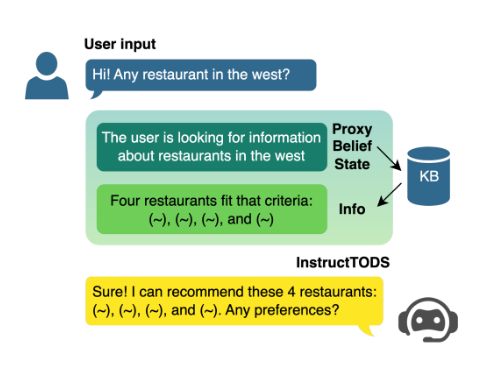
\includegraphics[width=0.5\textwidth]{InstructTODS}}
    \caption{معماری سیستم InstructTODS 
    \cite{chung2023instructtods}
    }
    \label{fig:InstructTODS}
\end{figure}


در این پژوهش، نویسندگان از مدل‌های زبانی بزرگ تنظیم شده با دستورالعمل برای ایجاد حالت باور استفاده می‌کنند که به عنوان نماینده‌ی نیت‌های کاربر عمل می‌کند و پایگاه‌های دانش را به صورت پویا در زبان طبیعی جستجو می‌کند. سپس اطلاعات بازیابی شده برای تولید پاسخ استفاده می‌شود. بر خلاف سیستم‌های سنتی وظیفه‌گرا که به مولفه‌های مجزا مانند طبقه‌بندی هدف و ردیابی وضعیت باور نیاز دارند، InstructTODS این فرآیندها را از طریق مدل‌های زبان بزرگ ادغام می‌کند و پاسخ‌ها را مستقیماً از ورودی‌های کاربر تولید می‌کند.
\newline
ارزیابی‌های جامع روی وظایف فرعی سیستم‌های گفتگو وظیفه‌گرا شامل ردیابی حالت گفتگو، طبقه‌بندی نیت، و تولید پاسخ نشان می‌دهد که InstructTODS عملکرد مشابهی با سیستم‌های 
کاملاً تنظیم‌شده%
\LTRfootnote{Fully fine-truned}
 دارد و حتی در شرایط صفر شات قادر است مکالمات را به طور مؤثر هدایت کند. همچنین، ارزیابی‌های انسانی نشان داده که از نظر مفید بودن، طبیعی بودن، و آموزنده بودن، InstructTODS از مدل‌های پیشرفته سیستم‌های گفتگو وظیفه‌گرا برتر است%
% Zhao-2023
\cite{madotto2021few}
.

جوانب مثبت پژوهش فوق به شرح زیر است:
\begin{itemize}
\item
قابلیت صفر شات: بدون نیاز به تنظیم دقیق یا داده‌های خاص وظیفه می‌توان از این سیستم استفاده کرد.
\item
تطبیق‌پذیری: توانایی کار با پایگاه‌های دانش متنوع بدون نیاز به مقادیر شکاف یا هستی‌شناسی‌های از پیش تعریف شده.
\item
کاهش هزینه‌های منابع: این رویکرد نسبت به سیستم‌های سنتی سیستم‌های گفتگو وظیفه‌گرا منابع کمتری نیاز دارد و کارایی را افزایش می‌دهد.
\item
گفتگوی طبیعی‌تر: بر اساس ارزیابی‌های انسانی، پاسخ‌های تولید شده طبیعی‌تر و مفیدتر هستند.
\end{itemize}

همچنین جوانب منفی این پژوهش نیز به شرح زیر است:
\begin{itemize}
\item
محدودیت‌های مدل‌های زبانی بزرگ: استفاده از مدل‌های زبانی بزرگ نیازمند منابع محاسباتی زیادی است که ممکن است در برخی موارد چالش‌برانگیز باشد.
\item
مشکلات بالقوه تعمیم: با اینکه روش صفر شات انعطاف‌پذیر است، ممکن است در وظایف خاص دامنه‌ای دچار مشکل شود.
\item
موارد شکست: در برخی از وظایف پیچیده‌تر، مدل ممکن است به درک زمینه‌ای بیشتری نیاز داشته باشد و شکست بخورد.
\end{itemize}

در %
\cite{madotto2021few}

، تمرکز بر شخصی‌سازی و نمایه‌سازی کاربر است تا سیستم‌های گفتگوی وظیفه‌محور به طور پویا بر اساس ترجیحات کاربر سازگار شوند. همچنین به چالش‌هایی مانند شروع سرد، حریم خصوصی، و امتیاز تعامل کاربر پرداخته‌‌شده است. برخلاف InstructTODS که بیشتر بر سازگاری عمومی و یادگیری صفر شات تمرکز دارد، رویکرد این تحقیق به شخصی‌سازی عمیق‌تر و تعامل کاربر با سیستم توجه ویژه‌ای دارد. استفاده از پروفایل کاربر به سیستم اجازه می‌دهد که پاسخ‌ها را با دقت بیشتری به نیازهای کاربر تنظیم کند، در حالی که InstructTODS بیشتر بر کارایی و سازگاری با پایگاه‌های دانش عمومی تکیه دارد. در حالی که هر دو سیستم به کاهش پیچیدگی در سیستم‌های گفتگو وظیفه را کمک می‌کنند، تفاوت اساسی در نحوه رسیدگی به نیازهای کاربران وجود دارد. رویکرد رساله فوق با تمرکز بر پروفایل کاربر، تجربه کاربر را بهینه می‌کند، در حالی که InstructTODS به انعطاف‌پذیری عمومی در تنظیمات مختلف توجه دارد.

\subsubsection{سیستم گفتگوی دامنه باز}
سیستم‌های گفتگوی دامنه باز برای درگیر شدن در گفتگو در مورد طیف گسترده‌ای از موضوعات بدون هدف یا هدف خاصی طراحی شده‌اند. برخلاف سیستم‌های وظیفه‌محور، که هدفشان دستیابی به یک نتیجه خاص (مانند رزرو پرواز یا ارائه پشتیبانی مشتری) است، سیستم‌های دامنه باز بر حفظ یک مکالمه طبیعی و روان تمرکز می‌کنند.


در % 
\cite{madotto2021few}
 ربات چند شات%
\LTRfootnote{Few-Shot Bot}
: یادگیری مبتنی بر پرامپت برای سیستم های گفتگو، سیستمی معرفی شده که بر مبنای یادگیری مبتنی بر پرامپت و چند شات طراحی شده است و به کمک چند نمونه مکالمه می‌تواند پاسخ‌های گفتگو محور را تولید کند. این سیستم بدون نیاز به تنظیم دقیق مدل و تنها با استفاده از پرامپت‌های محدود، قادر به مدیریت مکالمات مختلف است. این پژوهش به بررسی کاربردهای مختلف این رویکرد پرداخته و از جمله وظایف گفتگو، تولید پاسخ، پردازش مکالمات، و ایجاد پرسونا را ارزیابی کرده است. روش‌های مبتنی بر پرامپت به مدل‌های زبانی این امکان را می‌دهند که با بهره‌گیری از حداقل داده، عملکردی نزدیک به مدل‌های کاملاً آموزش‌دیده داشته باشند.
\newline
سهم اصلی این پژوهش، معرفی سیستم ربات چند شات است که از یادگیری چند شات مبتنی بر پرامپت بهره می‌برد تا به جای تنظیم دقیق و پرهزینه مدل‌های بزرگ زبانی، از چند نمونه مکالمه برای آموزش استفاده کند. این سیستم از توانایی یادگیری از طریق پرامپت‌ها بهره برده و با استفاده از مکانیزم 
انتخاب‌گر مهارت%
\LTRfootnote{Skill Selector}
، بهترین پاسخ را بر اساس تاریخچه مکالمات انتخاب می‌کند و از این طریق می‌تواند با جستجو در پایگاه‌های دانش پاسخ‌های طبیعی و مرتبط ارائه دهد.
\newline
دو چالش اصلی که در%
\cite{madotto2021few}
 به آن‌ها پرداخته شده عبارت‌اند از: 
\begin{enumerate}
\item
 هزینه بالای تنظیم و آموزش مدل‌های بزرگ زبانی: این مدل‌ها به منابع محاسباتی قابل‌توجهی نیاز دارند که باعث افزایش 
هزینه‌های عملیاتی و زمان‌بری فرایند آموزش می‌شود. این پژوهش تلاش کرده با استفاده از یادگیری چند شات مبتنی بر پرامپت، رویکردی کم‌هزینه و کارآمد ارائه دهد.
\item
نبود بنچمارک‌های رسمی برای ارزیابی روش‌های مبتنی بر پرامپت در سیستم‌های گفتگو: در این پژوهش، نویسندگان با بررسی یازده مجموعه داده مرتبط با مکالمات، یک بنچمارک رسمی برای یادگیری مبتنی بر پرامپت ارائه کرده‌اند که به ارزیابی عملکرد و مقایسه با روش‌های متداول کمک می‌کند.
\end{enumerate}

نویسندگان برای توسعه ربات چند شات از رویکردی استفاده کرده‌اند که در آن مدل‌های زبانی با نمونه‌های کوچک و بهینه‌شده هدایت می‌شوند. این سیستم از پرامپت‌های چند شات استفاده می‌کند و قادر است مکالمات متنوعی را مدیریت کرده و پاسخ‌های مناسبی ارائه دهد. از سوی دیگر، یک انتخاب‌گر مهارت به سیستم اضافه شده که بر اساس داده‌های ورودی، بهترین مهارت  مورد نیاز یک مکالمه را برای هر سوال انتخاب می‌کند. در این رویکرد، از هیچگونه تنظیم دقیق برای بهینه‌سازی مدل استفاده نمی‌شود و تنها پرامپت‌های کوتاه و ساده هدایتگر مدل هستند.

ارزیابی و نتایج پژوهش با استفاده از چندین معیار ارزیابی، از جمله تولید پاسخ‌های دقیق، پردازش پرسونا و ارزیابی‌های انسانی، نشان داده که ربات چند شات در بسیاری از موارد توانسته است به عملکردی مشابه یا بهتر از مدل‌های کاملاً تنظیم‌شده دست یابد. نتایج حاکی از آن است که این سیستم بدون نیاز به تنظیم دقیق و تنها با بهره‌گیری از پرامپت‌های چند شات، قادر به تولید پاسخ‌های طبیعی و مرتبط است که این رویکرد برای محیط‌هایی که نیاز به تنظیم دقیق و منابع زیاد ندارند، مناسب است.
\newline
از جمله مزایای اصلی این رویکرد، کاهش چشمگیر هزینه‌های محاسباتی است. به دلیل عدم نیاز به تنظیم دقیق و استفاده تنها از پرامپت‌ها، هزینه‌ها به میزان قابل‌توجهی کاهش یافته و این روش سازگاری مناسبی با وظایف مختلف مانند چت آزاد، تولید پاسخ‌های مبتنی بر دانش و پردازش اطلاعات دارد. همچنین، استفاده از انتخاب‌گر مهارت و یادگیری مبتنی بر پرامپت، باعث افزایش دقت پاسخ‌ها و تناسب آن‌ها با نیازهای کاربر می‌شود. 
\newline
از معایب این روش می‌توان به نیاز به طراحی دقیق پرامپت‌ها اشاره کرد که برای هر وظیفه نیازمند تخصص است. همچنین، در تعاملات پیچیده و شرایط خاص دامنه، این روش ممکن است دقت کمتری نسبت به مدل‌های کاملاً تنظیم‌شده داشته باشد.

پژوهش «XDAI: چارچوبی بدون تنظیم برای بهره‌برداری از مدل‌های زبانی از پیش آموزش‌دیده در تولید گفتگوی مبتنی بر دانش»%
\cite{yu2022xdai}
چارچوبی بدون نیاز به تنظیم دقیق ارائه می‌دهد که برای ایجاد سیستم‌های گفتگوی مبتنی بر دانش طراحی شده است. این سیستم از مدل‌های زبانی از پیش‌آموزش‌دیده استفاده می‌کند و تلاش می‌کند تا چالش‌های موجود در ساخت چنین سیستم‌هایی، از جمله گردآوری منابع دانش و نیاز به تنظیم مدل‌ها، را کاهش دهد. با استفاده از XDAI، توسعه‌دهندگان می‌توانند به سرعت سیستم‌های گفتگوی عمومی یا خاص دامنه ایجاد کنند. \\


مهم‌ترین نوآوری%
\cite{yu2022xdai}
 ارائه چارچوب XDAI است که شامل ویژگی‌های زیر است:
\begin{enumerate}
\item
 شروع سریع: ارائه یک سرویس گفتگوی مبتنی بر دانش که از منابع آماده برای دامنه عمومی استفاده می‌کند.
\item
 استنتاج کارآمد: استفاده از الگوهای پرسشی جدید که کیفیت دیالوگ‌ها را بدون نیاز به تنظیم دقیق مدل بهبود می‌بخشند.
\item
 استقرار سفارشی: امکان استفاده از افزونه‌های قابل تغییر برای جمع‌آوری خودکار منابع دانش خاص دامنه.
\item
 تغییرات افزایشی: ابزارهایی برای توسعه و شخصی‌سازی تدریجی سیستم فراهم می‌کند.
\end{enumerate}
در%
\cite{yu2022xdai}
 آزمایش‌های گسترده‌ای شامل ارزیابی‌های آنلاین و آزمون تورینگ انجام داده‌است و نتایج نشان می‌دهد که عملکردی رقابتی با مدل‌های پیشرفته کاملا تنظیم‌شده ارائه می‌دهد. همچنین قابلیت استفاده در دامنه‌های مختلف را با هزینه محاسباتی کمتر فراهم می‌کند.

از مزایای سیستم %
\cite{yu2022xdai}
 می توان به عدم نیاز به تنظیم دقیق و کاهش هزینه‌های محاسباتی و زمانی اشاره کرد. همچنین انعطاف‌پذیری بالا، قابلیت شخصی‌سازی و استفاده در دامنه‌های مختلف از نقاط قوت دیگر این سیستم است. علاوه بر موارد ذکرشده این سیستم ازشروع سرد پشتیبانی می کند که استفاده از قابلیت‌های شات صفر برای پاسخ‌دهی بدون نیاز به داده‌های اولیه آنرا میسر کرده است.\\

پژوهش ارایه‌شده در%
\cite{yu2022xdai}
 بر شخصی‌سازی، پروفایل‌سازی کاربران و همچنین ملاحضات حریم خصوصی تأکید دارد. در حالی که اXDAI با تمرکز بر یادگیری بدون تنظیم دقیق و تزریق دانش با پرامپت‌ها عملکردی کارآمدی ارائه می‌دهد، پژوهش رساله فوق قابلیت‌های بیشتری در زمینه تطبیق با کاربران و استفاده از پروفایل‌های کاربری برای تولید پاسخ‌های شخصی‌سازی‌شده دارد.

از معایب سیستم%
\cite{yu2022xdai}
می‌توان به کیفیت محدود پرامپت‌ها اشاره کرد. طراحی بهینه پرامپت‌ها برای وظایف پیچیده نیازمند تخصص است. همچنین عدم شخصی‌سازی عمیق را نیز می‌توان به عنوان عیب دیگری از این سیستم نام برد. در XDAI، تمرکز بیشتر بر بهره‌وری عمومی مدل‌ها و نه بر شخصی‌سازی عمیق پروفایل کاربر بوده است.


\subsection{تنظیم سریع و تکنیک های انطباق مدل}

\begin{enumerate}
\item
\textbf{تنظیم سریع برای کارایی سیستم گفتگو}

سیستم گفتگوی شخصی‌سازی‌شده با استفاده از تکنیک تنظیم سریع%
\cite{kasahara2022building}
 از روش‌های بهینه‌سازی 
بردارهای تعبیه‌شده%
\LTRfootnote{Embedding Vectors}
 برای پیش‌برد گفتگوها استفاده می‌کند. هدف اصلی این سیستم، ارائه پاسخ‌های گفتگو محوری است که هم از نظر 
پرسونا%
 \LTRfootnote{Persona}
(شخصیت از پیش تعریف شده) منسجم باشد و هم هزینه محاسباتی اندکی داشته باشد. این سیستم توانسته با به‌ حداقل رساندن تغییرات در پارامترهای اصلی مدل زبانی، کارایی مطلوبی از نظر منابع ارائه دهد.

این پژوهش به‌طور دقیق به چالش‌های 
سیستم‌های گفتگوی چند نوبتی%
\LTRfootnote{multi-turn dialogue system}
پرداخته و راه‌حل‌هایی برای بهبود شخصی‌سازی پاسخ‌ها بدون نیاز به داده‌های زیاد و قدرت محاسباتی ارائه می‌دهد. از جمله مشکلات اصلی که سیستم‌های چند نوبته با آن مواجه هستند، تناقض در پاسخ‌ها است؛ به عنوان مثال، ممکن است یک سیستم در مکالمه‌های مختلف مکان‌های متفاوتی را به عنوان محل سکونت خود اعلام کند. از طرف دیگر، سیستم‌های سنتی برای تعبیه اطلاعات شخصی در ورودی مدل، نیاز به طول ورودی زیادی دارند که کارایی را کاهش می‌دهد.
\newline
رویکرد % 
\cite{kasahara2022building}
 بر استفاده از تنظیم سریع تأکید دارد که با مسدود کردن پارامترهای مدل از پیش‌آموزش‌دیده و افزودن یک پرامپت با طول ثابت قبل از توالی ورودی، اطلاعات شخصیتی کاربر (پرسونا) را جاسازی می‌کند. 
\newline
این تکنیک از چند مولفه کلیدی تشکیل شده است:
\begin{itemize}
\item
مدل‌های زبانی از پیش‌آموزش‌دیده: استفاده از مدل‌های مبتنی بر معماری جی‌پی‌تی که از قبل قابلیت‌های گفتگوی عمومی دارند.
\item
تنظیم سریع: تنظیم تعداد کمی از بردارهای تعبیه‌شده که به خوبی می‌توانند اطلاعات شخصیت را ضبط و بهینه کنند.
\item
جاسازی اطلاعات شخصیت: این سیستم با استفاده از تعبیه‌های بهینه‌شده، اطمینان حاصل می‌کند که پاسخ‌ها با شخصیت خاص کاربر سازگار باشند.
\end{itemize}

کاساهارا و همکاران%
\cite{kasahara2022building}
 دو نوع ارزیابی خودکار و دستی را برای بررسی کیفیت سیستم ارائه داده‌اند. نتایج به زبان‌های انگلیسی و ژاپنی بررسی شده و نشان داده است که سیستم توانسته پاسخ‌هایی منسجم و طبیعی ارائه دهد. همچنین، کارایی محاسباتی سیستم در مقایسه با تنظیم دقیق کامل مدل به مراتب بالاتر است و نیاز به منابع محاسباتی کمتری دارد. مهم‌ترین معیارها در این ارزیابی‌ها شامل انسجام پاسخ‌ها بر اساس پرسونا، طبیعی بودن دیالوگ‌ها و کارایی محاسباتی بود که نتایج مطلوبی ارائه شد.

معماری روش پیشنهادی%
\cite{kasahara2022building}
 از چند لایه اصلی تشکیل شده است. ابتدا یک مدل زبانی از پیش‌آموزش‌دیده به عنوان هسته اصلی سیستم استفاده می‌شود. در این سیستم، پارامترهای مدل اصلی دست نخورده باقی می‌مانند و در عوض، یک پرامپت ثابت به ورودی مدل اضافه می‌شود که شامل اطلاعات مرتبط با شخصیت کاربر است. تنظیم سریع تنها بردارهای تعبیه‌شده مرتبط با پرامپت را بهینه می‌کند، بدون آنکه پارامترهای مدل اصلی تغییر کند. این رویکرد باعث می‌شود که سیستم بتواند با کمترین منابع، پاسخ‌هایی با توجه به شخصیت از پیش تعریف‌شده ارائه دهد.
معماری این سیستم در شکل
\ref{fig:Prompt-Tuning}
آورده شده‌است.

\begin{figure}[ht]
	\centerline{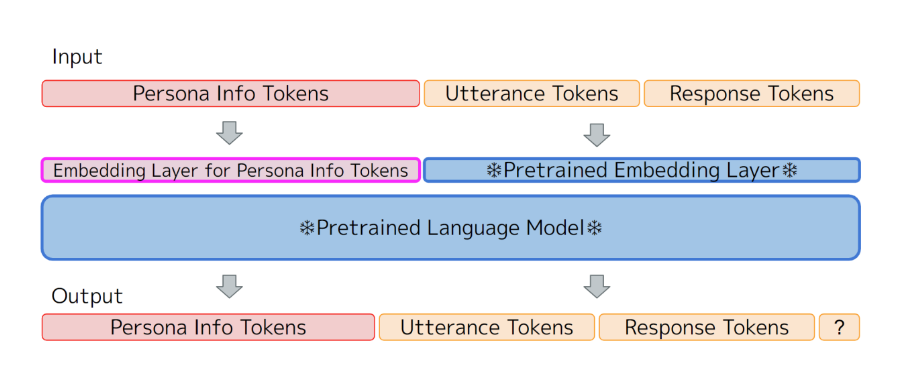
\includegraphics[width=0.8\textwidth]{8-Prompt-Tuning}}
		\caption{معماری ایجاد یک سیستم گفتگوی شخصی با تنظیم سریع 
			\cite{kasahara2022building}
	}
	\label{fig:Prompt-Tuning}
\end{figure}

مزایا و معایب سیستم به شرح زیر است.
\begin{itemize}
\item
مزایا:
\begin{itemize}
\item
کارایی محاسباتی بالا: به دلیل عدم نیاز به تغییر پارامترهای اصلی مدل، تنظیم سریع نسبت به تنظیم دقیق کامل منابع کمتری مصرف می‌کند.
\item
شخصی‌سازی با داده‌های اندک: با استفاده از داده‌های محدود (چند صد جفت گفتار-پاسخ)، سیستم می‌تواند پاسخ‌های شخصی ارائه دهد.
\item
اثربخشی بین‌المللی: سیستم در چندین زبان از جمله انگلیسی و ژاپنی عملکرد مطلوبی نشان داده‌است و از نظر زبانی قابل تطبیق است.
\item
سازگاری پرسونا: این سیستم توانسته به یکی از چالش‌های اصلی یعنی ثبات در پاسخ‌های شخصیتی به خوبی پاسخ دهد و از تضاد در مکالمات جلوگیری کند.
\end{itemize}


\item
معایب:
\begin{itemize}
\item
پیچیدگی در طراحی پرامپت: طراحی صحیح پرامپت‌ها برای هر شخصیت نیاز به تخصص دارد و اگر طراحی بهینه نباشد، ممکن است کیفیت دیالوگ کاهش یابد.
\item
محدودیت در انطباق‌پذیری: در حالی که این سیستم برای وظایف تعریف‌شده شخصیت محور عملکرد مطلوبی دارد، انعطاف‌پذیری آن در برخورد با شخصیت‌های متعدد یا وظایف پیچیده‌تر ممکن است محدود باشد.
\item
نبود مکانیزم شروع سرد: در این پژوهش به‌صراحت به مشکل شروع سرد اشاره‌ای نشده است؛ هرچند این تکنیک از طریق تنظیم سریع ممکن است برخی از مشکلات کمبود داده را کاهش دهد.
\end{itemize}
\end{itemize}
پژوهش ارائه‌شده، رویکردی کارآمد برای ایجاد سیستم گفتگوی شخصی‌سازی‌شده با استفاده از تنظیم سریع ارائه می‌دهد. این سیستم با حفظ ثبات شخصیت و مصرف حداقل منابع، توانسته است کارایی مطلوبی در چندین زبان ارائه دهد. در مقابل، تحقیقات رساله فوق به دنبال ارائه گفتگوهای هدف‌گرا و پروفایل‌سازی کاربر است که بتواند تجربه‌ای شخصی‌تر و مبتنی بر وظایف به کاربران ارائه دهد. این دو رویکرد می‌توانند در کنار یکدیگر مکمل باشند و بهبودهایی در زمینه شخصی‌سازی و انطباق‌پذیری گفتگوی هوشمند فراهم کنند.


\item
\textbf{تنظیم دقیق و رویکردهای ترکیبی}

 
دیلایت%
\LTRfootnote{DIALIGHT}
 توسعه سبک و چند زبانه و ارزیابی سیستم‌های گفتگوی وظیفه‌محور با مدل‌های زبانی بزرگ%
\cite{hu2024dialight}
، یک 
جعبه‌ابزار%
\LTRfootnote{Tool box}
 برای توسعه و ارزیابی سیستم‌های گفتگوی وظیفه‌محور چندزبانه ارائه می‌کند. این جعبه‌ابزار قابلیت مقایسه بین سیستم‌های مبتنی بر تنظیم دقیق مدل‌های زبانی از پیش آموزش دیده و سیستم‌های جدیدتر مبتنی بر مدل‌های زبانی بزرگ را دارد. دیلایت به کاربران این امکان را می‌دهد که علاوه بر ارزیابی‌های خودکار، از ارزیابی‌های انسانی دقیق در سطوح مختلف از جمله سطح گفتگو و سطح جمله نیز بهره‌مند شوند. همچنین این جعبه‌ابزار از یک معماری مبتنی بر میکروسرویس استفاده می‌کند که به مقیاس‌پذیری و کارایی بهتر کمک می‌کند 
\cite{hu2024dialight} \\
.

مشکل اصلی که در این پژوهش به آن پرداخته شده، چالش ارزیابی و توسعه‌ی کارآمد سیستم‌های گفتگوی وظیفه‌محور چندزبانه است. سیستم‌های کنونی عمدتاً بر مدل‌های زبانی از پیش آموزش دیده با تنظیم دقیق تکیه دارند که دقت بالاتری در تطبیق با وظایف خاص دارند، اما این مدل‌ها نیازمند زمان و منابع زیادی برای تنظیم هستند. از طرف دیگر، سیستم‌های مبتنی بر مدل‌های زبانی بزرگ از قابلیت تولید پاسخ‌های متنوع‌تر و طبیعی‌تر بهره‌مند هستند، اما مشکلاتی در اجرای دقیق دستورالعمل‌ها و تولید پاسخ‌های چندزبانه دارند.
\cite{hu2024dialight} \\
 دیلایت با ارائه‌ی یک جعبه‌ابزار جامع برای ارزیابی این دو رویکرد، شکاف موجود را برطرف می‌کند.

رویکرد اصلی دیلایت به شرح زیر است:
\begin{itemize}
\item
تنظیم دقیق مدل‌های مدل‌های زبانی از پیش آموزش‌دیده: دیلایت امکان تنظیم دقیق مدل‌های زبانی از پیش آموزش‌دیده برای تطبیق آن‌ها با وظایف خاص را فراهم می‌کند. این فرایند بر اساس آموزش مدل‌ها بر روی داده‌های مکالمه‌ی وظیفه‌محور انجام می‌شود.
\item
یادگیری درون‌زمینه%
\LTRfootnote{In-Context Learning}
 و بدون شات: سیستم‌های مبتنی بر مدل‌های زبان بزرگ بدون نیاز به تنظیم دقیق می‌توانند مکالمات وظیفه‌محور را در حالت‌های شات صفر و چندشات تولید کنند، اگرچه محدودیت‌هایی در تطابق دقیق با وظایف خاص دارند.
\item
پلتفرم چندزبانه: دیلایت امکان ارزیابی سیستم‌های گفتگو را در زمینه‌های تک‌زبانه، چندزبانه و حتی بین‌زبانی فراهم می‌کند و این یک قابلیت مهم برای توسعه‌ی سیستم‌های گفتگوی چندزبانه است.
\end{itemize}

ارزیابی‌ها نشان دادند که این روش منجر به دقت بالاتر و انسجام بیشتر در پاسخ‌ها می‌شود. 
اگرچه این سیستم‌ها خروجی‌های متنوعی تولید می‌کنند، اما در پیروی از دستورالعمل‌های خاص کار و ایجاد پاسخ‌های دقیق چندزبانه محدودیت‌هایی دارند. این مشکلات نشان‌دهنده نیاز به تحقیقات بیشتر در این حوزه است.

 مزایای این سیستم به شرح زیر است.
\begin{itemize}
\item
پشتیبانی از یادگیری بدون شات و درون‌زمینه: سیستم‌های مدل‌های زبانی بزرگ می‌توانند بدون نیاز به تنظیم دقیق، پاسخ‌های مورد انتظار در حالت‌های شات صفر و چندشات تولید کنند.
\item
ارزیابی چندزبانه و بین‌زبانی: دیلایت می‌تواند به‌صورت یکپارچه سیستم‌های گفتگوی وظیفه‌محور را در زبان‌های مختلف و حتی میان‌زبانی ارزیابی کند، که این یک نیاز مهم در توسعه سیستم‌های گفتگوی چندزبانه است.
\item
معماری مقیاس‌پذیر: استفاده از میکروسرویس‌ها امکان مقیاس‌پذیری بالا و کارایی بهتر را در ارزیابی‌ها فراهم می‌کند.
\item
ارزیابی جامع انسانی و خودکار: دیلایت با ترکیب ارزیابی‌های انسانی و خودکار دید جامعی از عملکرد سیستم‌ها ارائه می‌دهد.
\end{itemize}

همچنین از معایت دیلایت می توان به موارد زیر اشاره کرد.
\begin{itemize}
\item
مشکلات مدل‌های زبانی بزرگ در تطبیق با وظایف خاص: سیستم‌های مدل‌های زبانی بزرگ با چالش‌هایی در پای‌بندی دقیق به وظایف خاص و تولید پاسخ‌های منسجم مواجه هستند.
\item
مصرف منابع محاسباتی زیاد: استفاده از مدل‌های زبانی بزرگ برای سیستم‌های گفتگوی وظیفه‌محور منابع محاسباتی بالایی نیاز دارد.
\item
پیچیدگی تنظیم دقیق مدل‌های زبانی از پیش آموزش‌دیده: فرایند تنظیم دقیق مدل‌های زبانی از پیش آموزش دیده نیازمند منابع زیاد است، اما در مقایسه با مدل‌های زبانی بزرگ منجر به دقت و انسجام بیشتری در پاسخ‌ها می‌شود.
\end{itemize}

در مقایسه با روش ارایه‌شده رساله فوق، که بر شخصی‌سازی سیستم‌های گفتگو و حل مشکلات شروع سرد و حق فراموشی تمرکز دارد، دیلایت بیشتر به ارزیابی عملکرد سیستم‌های گفتگوی وظیفه گرا در زبان‌های مختلف و مقایسه بین روش‌های تنظیم دقیق مدل‌های زبانی از پیش آموزش دیده و مدل‌های زبان بزرگ پرداخته است. رساله فوق علاوه بر اینکه به یادگیری شات صفر و شخصی‌سازی مکالمات توجه دارد، به مشکلات حریم خصوصی و حق فراموشی نیز می‌پردازد که در دیلایت به‌طور خاص به آن پرداخته نشده است. \\

در %
\cite{samarinas2024simulating}
با عنوان «شبیه‌سازی گفتگوهای وظیفه‌گرا با استفاده از نمودارهای انتقال حالت و مدل‌های زبان بزرگ»، به معرفی 
سینتود%
\LTRfootnote{SynTOD}
 پرداخته است. این چارچوب نوآورانه برای تولید داده‌های مصنوعی طراحی‌شده که به توسعه و ارتقاء سیستم‌های گفتگوی وظیفه‌گرا کمک می‌کند. با استفاده از نمودارهای 
انتقال حالت%
\LTRfootnote{State Transition Graphs (STGs)}
 و مدل‌های زبانی بزرگ، سینتود مکالمات ساختاریافته‌ای را شبیه‌سازی می‌کند. مهم‌ترین ویژگی این چارچوب توانایی آن در تولید مجموعه داده‌های مصنوعی متنوع و غنی برای آموزش سیستم‌های گفتگو است که به مشکل کمبود داده‌های متنوع، که یکی از چالش‌های اصلی در آموزش مدل‌های گفتگو محور محسوب می‌شود، رسیدگی می‌کند.
در این پژوهش، سینتود به عنوان راه‌حلی برای تولید داده‌های مصنوعی معرفی شده که از جمع‌آوری داده‌های دنیای واقعی بی‌نیاز است. این چارچوب با استفاده از نمودارهای انتقال حالت به سیستم اجازه می‌دهد تا مکالمات را در قالب مسیرهای مشخص هدایت کند و سپس مدل‌های زبانی بزرگ این مسیرها را دنبال کرده و مکالمات وظیفه‌گرا تولید کنند. این مکالمات مصنوعی به بهبود عملکرد سیستم‌های گفتگویی، به ویژه در وظایف پیچیده نظیر طبقه‌بندی هدف، پر کردن شکاف و تولید پاسخ کمک می‌کنند.
\newline
یکی از چالش‌های اساسی که در طراحی سیستم‌های گفتگو وظیفه‌گرا مطرح است، کمبود داده‌های متنوع و باکیفیت برای آموزش این سیستم‌ها است. مدل‌های موجود به دلیل محدودیت‌های مرتبط با داده‌ها اغلب در انجام وظایف پیچیده مانند پاسخ‌دهی به سؤالات کاربران و دسته‌بندی مقاصد کاربران دچار مشکل هستند. روش‌های سنتی جمع‌آوری داده‌ها، مانند جمع‌سپاری، معمولاً پرهزینه و زمان‌بر هستند و نمی‌توانند حجم کافی از داده‌های لازم را برای توسعه سیستم‌های قوی فراهم کنند.
به علاوه، مدل‌های زبانی بزرگ که صرفاً برای تولید مکالمات استفاده می‌شوند، غالباً در ایجاد تنوع در مکالمات ناکام هستند و داده‌های تولید شده توسط آنها، پیچیدگی و عمق کافی برای انجام وظایف گوناگون را ندارند. سینتود با تولید مجموعه‌های داده مصنوعی از طریق ترکیب نمودارهای انتقال حالت و مدل‌های زبانی بزرگ، به این مشکل رسیدگی کرده و امکان تولید مکالمات متنوع و چندبعدی را فراهم می‌کند که در دامنه‌های مختلف وظیفه‌گرا قابل استفاده هستند.
\newline
سینتود با استفاده از نمودارهای انتقال حالت و 
پیاده‌روی‌های تصادفی%
\LTRfootnote{Random Walks}
 برای شبیه‌سازی مکالمات وظیفه‌گرا یک رویکرد جامع و ساختاریافته ارائه می‌دهد. 
مراحل این رویکرد به شرح زیر است:

\begin{itemize}
\item
نمودار انتقال حالت: در این بخش از سیستم، ساختار و جریان کلی مکالمه تعریف می‌شود. نمودار انتقال حالت نشان می‌دهد که یک کاربر از طریق مقاصد و نیازهای مختلف چگونه می‌تواند با سیستم تعامل کند. این نمودار جریان‌های مکالمه و پاسخ‌های سیستم به کاربران را در قالب حالات مختلف و گذرها به تصویر می‌کشد. نمودارهای انتقال حالت کمک می‌کنند تا مکالمات منطقی و پیش‌بینی‌پذیر طراحی شوند.
\item
پیاده‌روی‌های تصادفی: سینتود از پیاده‌روی‌های تصادفی برای پیمایش نمودارهای انتقال حالت استفاده می‌کند. این کار باعث می‌شود که سیستم بتواند مکالمات متنوع و چندگانه را تولید کند. هر بار که سیستم از یک نمودار عبور می‌کند، حالت‌های جدیدی در مکالمه به وجود می‌آیند که منجر به تولید مسیرهای متفاوت و متنوع می‌شود. این امر به سیستم امکان می‌دهد تا بتواند در شرایط مختلف، عملکردهای متفاوتی را به نمایش بگذارد.
\item
شبیه‌سازی پاسخ با مدل‌های زبان بزرگ: در مرحله نهایی، از مدل‌های زبان بزرگ تنظیم‌شده برای تولید پاسخ‌های طبیعی در مکالمات استفاده می‌شود. برخلاف روش‌های ساده که تنها به تولید یک پاسخ بر اساس یک ورودی می‌پردازند، در اینجا مدل‌های زبانی بزرگ از طریق شبیه‌سازی مکالمات در مسیرهای مختلف، پاسخ‌های ساختاریافته و مبتنی بر مکالمه تولید می‌کنند.
\end{itemize}

سینتود در دو دامنه مختلف مورد ارزیابی قرار گرفته است: کمک آشپزی و تجارت الکترونیک. در هر دو حوزه، عملکرد سینتود از طریق ارزیابی‌های خودکار و ارزیابی‌های انسانی مورد بررسی قرار گرفت. ارزیابی‌های خودکار شامل معیارهایی نظیر دقت و یادآوری بود که عملکرد سیستم را در انجام وظایف مختلف مانند طبقه‌بندی هدف و پر کردن شکاف‌ها بررسی کردند.
\newline
در کنار ارزیابی‌های خودکار، ارزیابی‌های انسانی نیز انجام شد تا کیفیت و انسجام مکالمات تولید شده توسط سیستم بررسی شود. نتایج نشان داد که سینتود قادر است مکالمات غنی‌تر و متنوع‌تری نسبت به مدل‌های ساده مبتنی بر یک ورودی ایجاد کند. به‌ویژه، مکالمات تولید شده توسط سینتود نسبت به مکالمات تک‌ورودی که توسط مدل‌های زبانی بزرگ تولید شده‌اند، بهبود قابل ملاحظه‌ای در عملکرد وظایف نشان دادند.

از مزایای سینتود می‌توان بهتولید داده‌های مصنوعی بدون نیاز به جمع‌آوری داده‌های واقعی اشاره کرد. 
یکی از بزرگ‌ترین مزیت‌های سینتود این است که نیازی به جمع‌آوری داده‌های واقعی و پرهزینه ندارد. با استفاده از مدل‌های زبان بزرگ و نمودارهای انتقال حالت، می‌توان داده‌های مصنوعی متنوع و با کیفیت بالا تولید کرد که در آموزش سیستم‌های گفتگو مورد استفاده قرار می‌گیرند.
\newline
همچنین مکالمات تولید شده توسط سینتود از نظر پیچیدگی و تنوع نسبت به مکالمات جمع‌آوری‌شده یا تولید‌شده توسط مدل‌های ساده‌تر، بسیار غنی‌تر هستند. این ویژگی به سیستم‌های گفتگو امکان می‌دهد تا در موقعیت‌های پیچیده عملکرد بهتری از خود نشان دهند.
علاوه بر این سینتود توانایی انطباق با دامنه‌های مختلف وظیفه‌محور را نشان داده است و در حوزه‌هایی نظیر تجارت الکترونیک و کمک آشپزی عملکرد موفقی داشته است.

از معایت سینتود می‌توان به وابستگی به طراحی نمودار انتقال حالت اشاره کرد. کیفیت گفتگوهای تولیدشده به میزان زیادی به طراحی دقیق نمودارهای انتقال حالت وابسته است. این به معنای آن است که برای هر دامنه، باید نمودارهای اختصاصی و متناسب طراحی شود که ممکن است نیاز به تنظیمات دستی و زمان‌بر داشته باشد.
\newline
در حالی که سینتود توانسته است در حوزه‌های محدود عملکرد موفقی از خود نشان دهد، گسترش این رویکرد به حوزه‌های متنوع‌تر و وسیع‌تر ممکن است چالش‌برانگیز باشد. به‌خصوص، مقیاس‌پذیری این رویکرد در دامنه‌های پیچیده‌تر نیاز به بررسی و آزمایش بیشتر دارد.


سینتود یک چارچوب نوآورانه است که با استفاده از نمودارهای انتقال حالت و مدل‌های زبان بزرگ، امکان تولید داده‌های مصنوعی غنی و متنوع برای آموزش سیستم‌های گفتگو را فراهم می‌کند. این رویکرد به‌ویژه در زمینه‌هایی که جمع‌آوری داده‌های واقعی دشوار است، بسیار مفید است. با این حال، شخصی‌سازی و پروفایل‌سازی کاربر در این چارچوب به‌صورت مستقیم مورد توجه قرار نگرفته است. در مقایسه، در تحقیقات این رساله، به‌طور خاص بر روی مسائل مربوط به شخصی‌سازی و مدیریت هویت گوینده تمرکز شده و تلاش می‌شود با استفاده از یادگیری چند‌شات و صفر‌شات و همچنین توسعه سیستم‌های گفتگوی وظیفه‌گرا یکی از چالش‌های اصلی در هوش مصنوعی است که هدف آن، طراحی سیستم‌هایی است که بتوانند به‌صورت دقیق و هوشمندانه به تعاملات کاربران در انجام وظایف خاص پاسخ دهند. با این حال، کمبود داده‌های متنوع و باکیفیت برای آموزش این سیستم‌ها، یکی از موانع بزرگ در بهبود عملکرد آنهاست. به همین دلیل، روش‌های جدید برای تولید داده‌های مصنوعی برای توسعه و آموزش این سیستم‌ها اهمیت ویژه‌ای پیدا کرده است.\\


سکوویچ و همکاران
\cite{sekulic2024reliable}
در پژوهش شبیه‌ساز کاربر مبتنی بر مدل‌های زبانی بزرگ قابل اعتماد برای سیستم‌های گفتگوی وظیفه‌گرا، به معرفی 
شبیه‌ساز کاربر آگاه از دامنه%
\LTRfootnote{Domain-aware user simulator}
 می‌پردازد. شبیه‌ساز کاربر آگاه از دامنه یک شبیه‌ساز مولد برای سیستم‌های گفتگوی وظیفه‌گرا است که از مدل‌های زبانی بزرگ استفاده می‌کند و با تنظیم دقیق آن‌ها بر داده‌های مکالمه‌ای خاص هر دامنه، به بهبود شبیه‌سازی کاربر می‌پردازد. هدف اصلی پژوهش، کاهش مشکلات مربوط به توهمات در شبیه‌سازی‌های کاربر و ایجاد تعاملات منسجم‌تر و مرتبط‌تر است که باعث افزایش دقت در شبیه‌سازی کاربران واقعی می‌شود. در نتیجه، شبیه‌ساز کاربر آگاه از دامنه ارزیابی و توسعه سیستم‌های گفتگو وظیفه‌گرا را به‌ویژه در تشخیص خطاها و دستیابی کاربران شبیه‌سازی‌شده به اهداف مشخص‌شده تسهیل می‌کند.
\newline
این پژوهش به مسئله عدم قابلیت اطمینان و ناسازگاری شبیه‌سازهای کاربر موجود می‌پردازد. روش‌های موجود معمولاً به سیستم‌های مبتنی بر قوانین سفت و سخت یا داده‌های حاشیه‌نویسی شده تکیه می‌کنند که منجر به تعاملات شبیه‌سازی‌شده نادرست و نامربوط می‌شوند. چالشی اصلی، توهمات شبیه‌ساز است که در آن سیستم محتوای نامرتبط یا متناقض تولید می‌کند. شبیه‌ساز کاربر آگاه از دامنه با کاهش توهمات و افزایش انسجام شبیه‌ساز با اهداف کاربر، به رفع این چالش می‌پردازد.
\newline
روش پیشنهادی شبیه‌ساز کاربر آگاه از دامنه شامل موارد زیر است:
\begin{itemize}
\item
تنظیم دقیق بر داده‌های دامنه‌محور: مدل‌های زبان بزرگ از طریق تنظیم دقیق بر روی مکالمات خاص دامنه‌ای، توانایی حفظ انسجام و مرتبط بودن مکالمات را افزایش می‌دهند.
\item
شبیه‌سازی مبتنی بر اهداف کاربر: شبیه‌ساز کاربر آگاه از دامنه با شروع از اهداف مشخص شده برای کاربر، با سیستم‌های گفتگوی وظیفه‌گرا تعامل می‌کند و دیالوگ‌های چندنوبتی ایجاد می‌کند.
\item
کاهش توهمات: تنظیم دقیق شبیه‌ساز کاربر آگاه از دامنه بر داده‌های خاص هر دامنه به کاهش توهمات کمک می‌کند و پاسخ‌های مرتبط‌تر و با دقت بیشتری را تولید می‌کند.
\item
تشخیص خطا: شبیه‌ساز کاربر آگاه از دامنه برای شناسایی خطاهای رایج در سیستم‌های گفتگوی وظیفه‌گرا طراحی شده است، که این امر باعث بهبود دقت و عملکرد سیستم می‌شود.
\end{itemize}

شبیه‌ساز کاربر آگاه از دامنه با استفاده از دو معیار معتبر در ارزیابی سیستم‌های گفتگوی وظیفه‌گرا مورد آزمایش قرار گرفته است. نتایج نشان می‌دهند که تنظیم دقیق مدل‌های زبانی بزرگ بر روی داده‌های خاص دامنه‌ای، انسجام بیشتری با اهداف کاربران فراهم می‌کند و توهمات را کاهش می‌دهد.

دستاوردهای کلیدی ارزیابی شامل موارد زیر است:
\begin{itemize}
\item
بهبود تحقق اهداف کاربر: شبیه‌ساز کاربر آگاه از دامنه منجر به تعاملات موفق‌تری شد که در آن کاربران شبیه‌سازی شده به اهداف تعیین‌شده خود رسیدند.
\item
کاهش توهمات: مدل‌های زبانی بزرگ  تنظیم شده کمتر مستعد تولید پاسخ‌های نامرتبط و نامنسجم بود.
\item
تنوع واژگانی: شبیه‌ساز کاربر آگاه از دامنه با ارائه تنوع زبانی در دیالوگ‌های شبیه‌سازی شده، اما در مقایسه با روش‌های یادگیری درون‌زمینه‌ای، کمی تنوع کمتری دارد.
\end{itemize}
از مزایای این سیستم می‌توان به انطباق ویژه دامنه اشاره کرد. تنظیم دقیق بر روی داده‌های دامنه‌محور، مکالمات منسجم‌تر و مرتبط‌تری را تولید می‌کند. همچنین تمرکز شبیه‌ساز کاربر آگاه از دامنه بر انسجام مکالمات باعث کاهش توهمات می‌شود و پاسخ‌های قابل اعتمادتر و دقیق‌تری ارائه می‌دهد.شبیه‌ساز کاربر آگاه از دامنه نیازی به دسترسی به عملکرد داخلی یا سیاست‌های سیستم ندارد، که آن را به یک راه‌حل منعطف تبدیل می‌کند. این شبیه‌ساز قادر به تشخیص خطاهای رایج در سیستم‌های گفتگوی وظیفه‌گرا است و به بهبود عملکرد کلی سیستم کمک می‌کند.
\newline
از معایب سیستم 
\cite{sekulic2024reliable}
 می توان به پیچیدگی محاسباتی اشاره کرد. تنظیم دقیق مدل‌های زبان بزرگ به قدرت محاسباتی زیادی نیاز دارد و ممکن است هزینه‌بر باشد.
همچنین تنوع واژگانی محدود از دیگر نقاط ضعف آن است. اگرچه شبیه‌ساز کاربر آگاه از دامنه تنوع زبانی را فراهم می‌کند، اما در مقایسه با روش‌های یادگیری درون‌زمینه‌ای، تنوع کمتری دارد. شبیه‌ساز کاربر آگاه از دامنه بر اهداف وظیفه‌محور متمرکز است و از نمایه‌سازی کاربر یا شخصی‌سازی استفاده نمی‌کند.

در مقایسه با روش ارایه‌شده در این رساله که بر شخصی‌سازی، نمایه‌سازی کاربر و حل مشکل شروع سرد تأکید دارد، تمرکز 
\cite{sekulic2024reliable}
 شبیه‌ساز کاربر آگاه از دامنه  بر کاهش توهمات و شبیه‌سازی وظیفه‌محور است. در حالی که هر دو از مدل‌های زبانی بزرگ استفاده می‌کنند، شبیه‌ساز کاربر آگاه از دامنه  بر تنظیم دقیق دامنه‌محور تمرکز دارد، در حالی که روش رساله فوق بر تنظیم سریع و استفاده از یادگیری چند‌شات برای افزایش انطباق سیستم بدون نیاز به تنظیم دقیق گسترده تأکید دارد.

\end{enumerate}

\subsection{پروفایل کاربری}
\subsubsection{تکنیک های پروفایل صریح و ضمنی}
پروفایل صریح به اطلاعاتی اشاره دارد که به‌صورت واضح و مستقیم از کاربران جمع‌آوری می‌شود. این اطلاعات معمولاً شامل وابستگی‌ها، علایق و نیازهای کاربر است که به‌طور مستقیم از طریق پرسشنامه‌ها، نظرسنجی‌ها یا تنظیمات حساب کاربری به‌دست می‌آید. اطلاعات به‌‌دست آمده، مستقیماً مربوط به خواسته‌ها و نظرات کاربر است لذا به آسانی قابل اندازه گیری هستند %
\cite{jabeenuser}
.
\newline
پروفایل ضمنی به اطلاعاتی اشاره دارد که به‌طور غیرمستقیم از رفتارها و فعالیت‌های کاربران در پلتفرم‌ها جمع‌آوری می‌شود. این اطلاعات از مرور رفتار کاربر، کلیک‌ها و تعاملات او به‌دست می‌آید. این داده‌ها از طریق رفتار کاربری مانند تاریخچه جستجو و خریدها جمع‌آوری می‌شود %
\cite{jabeenuser}
. 
\newline

بوکلیش و همکاران %
\cite{azzam2022model}
 ،
 یک رویکرد مبتنی بر یادگیری ماشینی برای پروفایل کاربر را با تجزیه و تحلیل داده‌های رسانه‌های اجتماعی آنلاین برای شناسایی اولویت‌ها، جزئیات جمعیت‌شناختی و رفتارهای کاربران بررسی می‌کند. ایده اولیه این پژوهش مدلی است که از تکنیک‌های رگرسیون برای استخراج پروفایل‌های کاربر بر اساس سن، جنسیت و سایر ویژگی‌ها و پیش‌بینی معیارهای تعامل، مانند تعداد لایک‌های پست، بر اساس فعالیت کاربر در پلتفرم‌های رسانه‌های اجتماعی مانند فیس‌بوک استفاده می‌کند. این مدل با تجزیه و تحلیل داده های صریح (سن، جنسیت) و ضمنی (پست ها، لایک ها، اشتراک گذاری ها) به ایجاد بینش کاربر کمک می کند.

پروفایل‌سازی کاربر که بر اساس تجزیه و تحلیل رسانه‌های اجتماعی انجام می‌شود، چالش‌هایی را در مدیریت و تحلیل مؤثر داده‌های گسترده و بدون ساختار این پلتفرم‌ها به همراه دارد. با افزایش حجم اطلاعات تولید شده توسط کاربران، پیش‌پردازش داده‌ها و شناسایی الگوهای رفتاری کاربران برای ایجاد پروفایل‌های دقیق، به‌ویژه در زمینه‌هایی مانند سیستم‌های توصیه‌گر و بازاریابی هدفمند، ضروری است. در این مدل، استفاده از تکنیک‌های رگرسیون برای تحلیل روابط میان داده‌های جمعیت‌شناختی و رفتارهای اجتماعی کاربر (مانند لایک کردن یا اشتراک‌گذاری) به منظور پیش‌بینی معیارهای تعامل و همچنین ایجاد پروفایل‌های شخصی به کار گرفته می‌شود.\\


سهم اصلی 
\cite{azzam2022model}
 توسعه یک مدل یادگیری ماشینی برای پروفایل کردن کاربران بر اساس فعالیت‌های رسانه‌های اجتماعی آن‌ها است که در درجه اول بر داده‌های فیس‌بوک تمرکز دارد. با استفاده از تجزیه و تحلیل داده های رسانه های اجتماعی، هدف نویسندگان پیش بینی تعامل و ترجیحات کاربر، پرداختن به چالش استخراج بینش ارزشمند از داده های گسترده، پویا و بدون ساختار در شبکه های اجتماعی است. این وظیفه در زمینه هایی مانند سیستم های توصیه کننده، بازاریابی هدفمند و تجزیه و تحلیل احساسات مرکزی است.
چالش در مدیریت و تجزیه و تحلیل موثر داده‌ها در دسته‌های مختلف، زیرمجموعه‌ها و تعاملات کاربر، مانند پست‌ها، لایک‌ها و اشتراک‌گذاری‌ها در مقیاس بزرگ است. با توجه به حجم و تنوع داده‌های اجتماعی، پیش پردازش و شناسایی نمایش‌های دقیق کاربر بر اساس داده‌های صریح (مانند سن، جنسیت) و داده‌های ضمنی (مانند رفتار کاربر) برای استخراج نمایه‌های دقیق و جامع کاربر حیاتی است.

رویکرد پیشنهادی شامل استفاده از یک مدل رگرسیون به عنوان یک ابزار پیش بینی است که رفتار کاربران را بر اساس سن، جنسیت و سایر عوامل جمعیت شناختی ارزیابی می کند. داده‌های فیس‌بوک، به‌ویژه تعاملات کاربر (لایک کردن، اشتراک‌گذاری، نظر دادن)، برای ایجاد یک مدل نمایه کاربر استفاده شد. این مطالعه از تجزیه و تحلیل داده‌های اکتشافی و تکنیک‌های رگرسیون استفاده می‌کند و یک رگرسیون تولید می‌کند که معیارهای تعامل مانند تعداد لایک‌هایی که ممکن است پست‌های کاربر دریافت کند را پیش‌بینی می‌کند. این مدل با استفاده از خطای 
آر-اسکورد%
\LTRfootnote{R-squared}
برای تعیین دقت و اثربخشی پیش‌بینی آن ارزیابی می‌شود.
\newcommand{\RLnum}[1]{#1} % Simply outputs the Persian numerals directly
\newcommand{\num}[1]{%
   \LR{\hspace{0pt}#1\hspace{0pt}}
}

عملکرد پیش‌بینی مدل با استفاده از معیار خطای آر-اسکورد سنجیده شده است و نتیجه نرخ خطای \num{۰.۱۹۹} به دست آمد. 
این عدد نشان می‌دهد که مدل تا حدی قابل قبول عمل کرده است، اما همچنان جای پیشرفت وجود دارد. بررسی نتایج نشان می‌دهد که استفاده از پروفایل‌های مبتنی بر رگرسیون می‌تواند بینش‌های مفیدی درباره الگوهای رفتار کاربران از طریق داده‌های موجود در فعالیت‌های رسانه‌های اجتماعی ارائه دهد. به بیان ساده‎تر، این مدل می‌تواند به ما کمک کند الگوها و رفتارهای کلی کاربران را بهتر درک کنیم.

اما در این مسیر، چالش‌هایی نیز وجود دارد. به عنوان مثال، درک دقیق احساسات کاربران یا تشخیص سطوح ظریف تعامل آن‌ها کار ساده‌ای نیست. این نوع الگوها اغلب پیچیده‌تر هستند و نیازمند رویکردهای پیشرفته‌تری برای تحلیل دقیق‌تر هستند%
\cite{azzam2022model}
. بنابراین، هرچند مدل فعلی می‌تواند نقطه شروع خوبی باشد، اما برای رسیدن به دقت بالاتر، توسعه روش‌های جدید و بهینه‌سازی بیشتر ضروری به نظر می‌رسد.


مزایای %
\cite{azzam2022model}
 به شرح زیر است.
\begin{itemize}
\item
کارایی در تولید پروفایل: این مدل می‌تواند به سرعت پروفایل‌هایی را بر اساس داده‌های اولیه جمعیت‌شناختی و رفتاری ایجاد کند و از وظایفی مانند بازاریابی هدفمند و تحلیل احساسات پشتیبانی کند.
\item
قابلیت اجرا در سراسر دامنه‌ها: پروفایل کاربری از طریق این مدل کاربردهای بالقوه ای در زمینه‌های مختلف دارد، مانند نظارت بر سلامت روان، بازاریابی شخصی و تجزیه‌وتحلیل رفتار مجرمانه.
\item
پروفایل صریح و ضمنی: این رویکرد داده‌های جمعیتی صریح را با بینش‌های مبتنی بر رفتار ضمنی ترکیب می‌کند، که اجازه می‌دهد تا نمایه کاربر دقیق‌تری داشته باشد.
\end{itemize}
از معایب این روش می توان به موارد زیر اشاره کرد.
\begin{itemize}
\item
پیچیدگی محدود: اتکای مدل به رگرسیون ساده ممکن است ظرفیت آن را برای ثبت روندهای رفتاری متفاوت، به ویژه در تطبیق داده بالا، محدود کند.
\item
وابستگی به داده‌های رسانه‌های اجتماعی: این مدل به‌شدت به دقت و دردسترس‌بودن داده‌های رسانه‌های اجتماعی متکی است، که ممکن است همیشه برای نمایه‌سازی جامع قابل اعتماد یا کافی نباشد.
\end{itemize}


در مقایسه با %
\cite{azzam2022model}
، تحقیقات پژوهش فوق بر توسعه یک سیستم گفتگوی شخصی متمرکز است که از پروفایل کاربر برای توصیه‌ها و تعاملات متناسب استفاده می‌کند. مولفه پروفایل کاربری همچنین شامل نمایه‌سازی ضمنی و صریح است، اما فراتر از داده‌های جمعیت‌شناختی ثابت است و شامل تجزیه و تحلیل احساسات پویا و روش‌های فیلتر مشارکتی، مانند فیلتر مشارکتی مبتنی بر آیتم می‌شود. علاوه بر این، سیستم فوق بر حل مشکل شروع سرد با ایجاد نمایه‌های کاربر اولیه بر اساس داده‌های تعامل محدود و ارائه یک تجربه شخصی از طریق تنظیم سریع با کمک یک مدل زبان بزرگ تأکید می‌کند.

در حالی که هر دو رویکرد از نمایه‌سازی استفاده می کنند، روش پیشنهادی رساله فوق با ادغام اصل حق فراموشی فراتر می‌رود و به کاربران اجازه می‌دهد تا درخواست حذف داده‌های خود را از سیستم کنند. این با مقررات حفظ حریم خصوصی مطابقت دارد، که به طور مستقیم در مدل پروفایل کاربری از تجزیه و تحلیل رسانه های اجتماعی به آن پرداخته نمی شود. علاوه بر این، تحقیق فوق به جای تکیه بر پیش‌بینی‌های مبتنی بر رگرسیون، از تنظیم دقیق و یادگیری چند شات برای بهبود سازگاری مدل و مدیریت تعاملات شخصی در یک محیط گفتگوی وظیفه‌محور استفاده می‌کند.

به طور خلاصه، در حالی که نمایه‌سازی کاربر از طریق تجزیه‌وتحلیل رسانه‌های اجتماعی بینش‌های ارزشمندی را در مورد نمایه سازی اولیه کاربر از داده های اجتماعی ارائه می دهد، هدف تحقیق فوق گسترش این قابلیت‌ها با شخصی‌سازی پیچیده، رعایت حریم خصوصی، و تعاملات سازگار با کاربر با استفاده از تکنیک‌های پیشرفته یادگیری‌ماشینی است.\\


نگ و همکاران %
\cite{nag2023knowledge}، 
 به بررسی چگونگی تحلیل و ایجاد پروفایل کاربران از داده‌های متنی چندزبانه که در رسانه‌های اجتماعی منتشر می‌شوند، می‌پردازد. هدف اصلی این مطالعه، توسعه مدلی برای تحلیل و پروفایل‌سازی کاربران بر اساس زبان‌ها و موضوعات مختلفی است که در این پلتفرم‌ها استفاده می‌شود. روش پیشنهادی با بهره‌گیری از تکنیک‌های مختلف پردازش زبان طبیعی و استفاده از منابع دانش‌بنیان همچون 
وردنت%
\LTRfootnote{WordNet}
، تلاش می‌کند که احساسات و موضوعات پنهان در پس متون چندزبانه را شناسایی و تحلیل کند.

مشکل اصلی در
\cite{nag2023knowledge}
، تحلیل و شناسایی احساسات و موضوعات مرتبط با متن‌های چندزبانه است. کاربران در پلتفرم‌های اجتماعی از زبان‌های مختلفی برای ابراز نظرات خود استفاده می‌کنند، که تحلیل این متن‌ها و شناسایی اطلاعات مرتبط را برای ماشین‌ها به چالش می‌کشد. چالش دیگر، دسترسی به منابع و پایگاه‌های‌داده مرتبط و آماده‌سازی آن‌ها برای استفاده در مدل یادگیری ماشین است.


رویکرد پیشنهادی شامل سه مرحله اصلی است:
\begin{enumerate}
\item
تشخیص زبان: در مرحله اول، زبان هر کلمه با استفاده از مقایسه 
یونیکد%
\LTRfootnote{UNICODE}
 و فهرستی از زبان‌های مختلف شناسایی می‌شود. سپس کل متن به زبان هدف (در این آزمایش، انگلیسی) ترجمه می‌شود.
\item
تحلیل احساسات: در این مرحله، با استفاده از مجموعه داده‌ای شامل کلمات با بار معنایی مثبت و منفی، احساسات متن شناسایی می‌شود. این مجموعه داده شامل ۴۰۰۰+ کلمه مثبت و ۴۰۰۰+ کلمه منفی از پایگاه داده 
کگل%
\LTRfootnote{Kaggle - https://www.kaggle.com/}
جمع‌آوری شده است.
\item
شناسایی موضوع: در مرحله نهایی، موضوع متن با استفاده از آرشیو روزنامه و وردنت شناسایی می‌شود. این آرشیو با استفاده از منابع آنلاین و سلسله‌مراتب واژگان وردنت ایجاد می‌شود که به شناسایی کلمات مرتبط با موضوعات مختلف تا سطح سوم کمک می‌کند.
\end{enumerate}
این مدل بر روی 200 پیام در ده زبان مختلف آزمایش شده است.
نتایج نشان داد که مدل پیشنهادی با دقت قابل قبولی می‌تواند احساسات و موضوعات متون را در زبان‌های مختلف شناسایی کند. هرچند، چالش‌هایی همچون پیچیدگی ترجمه‌های چندزبانه و نیاز به داده‌های آموزشی بیشتر برای بهبود عملکرد مدل نیز ذکر شده‌است.\\

این مدل می‌تواند احساسات و موضوعات را در چندین زبان تحلیل کند که آن را برای پروفایل‌سازی کاربران در محیط‌های چندزبانه مناسب می‌سازد.
همچنین این مدل با استفاده از وردنت و آرشیو روزنامه‌ها و استفاده از منابع دانش بنیان برای استخراج موضوعات متن، به بهبود تحلیل کمک می‌کند.

از معایت این روش نیاز باید به پردازش و پیش‌پردازش پیچیده اشاره کرد. فرآیند پیش‌پردازش داده‌ها و ترجمه متون چندزبانه نیازمند زمان و منابع است. همچنین ترجمه اتوماتیک به زبان هدف (انگلیسی) ممکن است معانی دقیق را در برخی از متون از دست بدهد که دقت تحلیل را تحت تاثیر قرار می‌دهد.

در مقایسه با پژوهش این رساله،
\cite{nag2023knowledge}
 تمرکز بیشتری بر پروفایل‌سازی بر اساس داده‌های چندزبانه دارد و از منابع خارجی همچون وردنت و داده‌های خبری برای شناسایی موضوعات استفاده می‌کند. در تحقیق این رساله، پروفایل‌سازی کاربر فراتر از اطلاعات صریح و احساسات متنی کاربران است و با استفاده از تحلیل احساسات و فیلترسازی مشارکتی، نمایه‌سازی دقیق‌تر و شخصی‌سازی شده‌ای از کاربران برای تعاملات گفتگو محور ارائه می‌شود.



\subsubsection{تحلیل احساسات و فیلتر کردن مبتنی بر آیتم}
تحلیل احساسات و فیلتر کردن مبتنی بر آیتم دو تکنیک مهم در سیستم‌های توصیه‌گر و پروفایل سازی کاربر هستند که به کمک آن‌ها می‌توان به طور مؤثری به پیش‌بینی تعاملات کاربران و ارائه پیشنهادات مناسب پرداخت. 
تحلیل احساسات فرآیندی است که به شناسایی و استخراج احساسات و نظرات کاربران از متون می‌پردازد. این متون می‌توانند شامل نظرات، نقدها، توییت‌ها و دیگر اشکال ارتباطی باشند. همچنین فیلترکردن مبتنی بر آیتم یک روش برای پیشنهاد دادن آیتم‌ها به کاربران بر اساس تعاملات قبلی آن‌ها با آیتم‌های مشابه است.


پترسون و همکاران %
\cite{peterson2021user}،
 یک رویکرد متمرکز بر افزایش روش‌های پروفایل کاربر برای بهبود توصیه‌ها در سیستم‌های توصیه‌گر ارائه می‌کند. این بر اهمیت پروفایل‌های پویا و دقیق کاربر در مقابله با اضافه بار اطلاعات تاکید می‌کند، چالشی رو به رشد زیرا پلتفرم‌های بیشتری حجم زیادی از محتوا را ارائه می‌دهند. این پژوهش دو روش کلیدی پروفایل را بررسی می‌کند: یک چارچوب پروفایل کاربری سلسله مراتبی و یک رویکرد پروفایل کاربر مبتنی بر برچسب که از نظریه بازی برای متعادل‌کردن ویژگی‌ها در نمایش پروفایل استفاده می‌کند.

سهم اصلی \cite{peterson2021user}، بررسی رویکردهای نوآورانه پروفایل کاربر در سیستم‌های توصیه‌گر برای بهبود دقت توصیه است. پروفایل کاربری برای سیستم‌های توصیه‌گر برای ایجاد توصیه های مرتبط که تجربه کاربر را غنی می‌کند و اضافه بار اطلاعات را کاهش می‌دهد بسیار مهم است. این کار در درجه اول به چالش ایجاد نمایه‌های کاربری قوی می‌پردازد که به‌طور دقیق علایق کاربر را در سطوح چندگانه منعکس می‌کند، و سیستم‌های توصیه‌گر را قادر می‌سازد تا محتوای متناسب و مرتبط را به طور کارآمد ارائه دهند.

مشکل بر روی ساختن پروفایل هایی متمرکز است که نه تنها علایق کاربر را به طور دقیق منعکس می‌کند، بلکه به صورت پویا با تغییرات رفتار کاربر تنظیم می‌شود. سیستم‌های توصیه‌گر سنتی اغلب با ایجاد پروفایل‌هایی که جزئیات و کلیات را متعادل می‌کند، مشکل دارند و بر ظرفیت آنها برای ارائه توصیه‌های مناسب تأثیر می‌گذارد. تمرکز این پژوهش بر چارچوب‌های پروفایل سلسله مراتبی و مبتنی‌بر برچسب، بینش‌هایی را برای دستیابی به این تعادل ارائه می‌دهد.

پترسون و همکاران در 
\cite{peterson2021user}
دو روش اصلی برای پروفایل کاربری را بررسی می‌کنند:
\begin{itemize}
\item
چارچوب پروفایل کاربری سلسله مراتبی: این رویکرد نشان‌دهنده علایق کاربر در سطوح مختلف جزئیات است. این یک ساختار لایه‌ای برای علایق کاربر ایجاد می‌کند و به سیستم‌های توصیه‌گر اجازه می‌دهد اولویت‌های کاربر را از دسته‌های گسترده تا موارد خاص درک کند. این چارچوب انعطاف‌پذیری را افزایش می‌دهد و سیستم را قادر می‌سازد تا توصیه‌هایی را در دسته‌های مختلف و جزئیات ارائه دهد.
\item
پروفایل کاربری مبتنی بر برچسب با استفاده از تئوری بازی: در این روش، تئوری بازی برای مدیریت مبادله بین ویژگی و عمومیت در پروفایل های کاربر استفاده می شود. برچسب‌های مرتبط با تعاملات کاربر وزن می‌شوند تا ارتباط آنها را منعکس کنند، بنابراین نمایه را اصلاح می‌کنند. تئوری بازی برای بهینه‌سازی این فرآیند استفاده می‌شود و اطمینان حاصل می‌کند که پروفایل‌ها نه خیلی وسیع و نه بیش از حد جزئی هستند و به توصیه‌های کارآمد و دقیق اجازه می‌دهند.
\end{itemize}
پترسون و همکاران
\cite{peterson2021user}
اثربخشی این روش ها را با تجزیه و تحلیل توانایی آنها در بهبود دقت توصیه ها و رضایت کاربر ارزیابی می کند. چارچوب سلسله مراتبی نشان داده شده است که انعطاف پذیری در سیستم‌های توصیه‌گر را فراهم می کند و با زمینه های مختلف توصیه سازگار می شود. در همین حال، تکنیک پروفایل‌سازی مبتنی بر برچسب دقت بهبود یافته‌ای را در تطبیق علایق کاربر با موارد موجود نشان می‌دهد. هر دو رویکرد در نهایت به یک فرآیند توصیه اصلاح‌شده کمک می‌کنند، و به طور موثر به مسئله اضافه بار اطلاعات رسیدگی می‌کنند.


از جوانب مثبت%
\cite{peterson2021user}
 باید به انعطاف‌پذیری و دقت این روش اشاره کرد. ساختار سلسله مراتبی اجازه می‌دهد تا توصیه‌هایی در سطوح مختلف دانه‌بندی ارائه شود و سازگاری با نیازهای کاربر بهبود یابد. همچنین روش پروفایل‌سازی مبتنی بر نظریه بازی تضمین می‌کند که پروفایل‌ها نه بیش از حد عمومی هستند و نه خیلی خاص، که منجر به توصیه‌های مرتبط‌تر می‌شود. هر دو رویکرد به سیستم‌های توصیه‌گر اجازه می‌دهند تا به علایق کاربر در حال تکامل پاسخ دهند و پروفایل ها را به‌روز و موثر نگه دارند.

از معایب 
\cite{peterson2021user}
 می توان به پیچیدگی پیاده‌سازی آن اشاره کرد. توسعه یک چارچوب سلسله مراتبی چند سطحی و اجرای نظریه بازی برای وزن‌دهی برچسب می‌تواند از نظر محاسباتی پیچیده باشد. همچنین پتانسیل ایجاد نویز در برچسب‌ها زیاد است. روش مبتنی بر برچسب به ارتباط دقیق برچسب متکی است و تگ‌های پر سروصدا یا نامربوط می توانند بر دقت پروفایل تأثیر بگذارند.

در مقایسه با تمرکز تحقیقاتی فعلی، که شامل پروفایل کاربری در سیستم‌های گفتگو می‌شود، رویکرد پترسون و همکاران بیشتر بر روی سیستم‌های توصیه‌گر برای مدیریت اضافه بار اطلاعات متمرکز است. در حالی که تحقیقات موجود بر شخصی‌سازی و نمایه‌سازی کاربر نیز تأکید می‌کند، تکنیک‌های اضافی مانند فیلترکردن مشارکتی و تجزیه و تحلیل احساسات را که به‌ویژه برای سیستم‌های گفتگو طراحی شده است، در خود جای داده است.

در تحقیقات سیستم گفتگو، شخصی‌سازی نه تنها از طریق نمایه‌سازی، بلکه از طریق تولید پاسخ پویا بر اساس تاریخچه تعامل کاربر و بازخورد ضمنی حاصل می‌شود که در پژوهش متمرکز بر سیستم‌های توصیه‌گر کمتر بر آن تأکید شده‌است. علاوه بر این، سیستم گفتگو حق فراموش شدن را در اولویت قرار می‌دهد و به حفظ حریم خصوصی و حفظ داده‌ها می پردازد - حوزه هایی که در این پژوهش پوشش داده نمی شوند.

به طور خلاصه، روش‌های نمایه‌سازی در 
\cite{peterson2021user}
، دقت توصیه‌ها و تجربه کاربر را با تأکید بر نمایش منافع چند سطحی و تعادل بهینه در استفاده از برچسب، افزایش می‌دهد. در مقابل، تحقیق فعلی بر ادغام پروفایل کاربر با شخصی‌سازی گفتگوی بلادرنگ تمرکز دارد و شامل یک چارچوب قوی برای حفظ حریم خصوصی داده‌ها است که آن را به یک رویکرد جامع‌تر برای سیستم‌های تعامل کاربر محور تبدیل می‌کند.

\subsubsection{تکنیک های پروفایل سازی کاربر برای افزایش حریم خصوصی}
ژنگ و همکاران %
\cite{zhang2024right}
  به بررسی و تحلیل مفهوم حق فراموشی در زمینه مدل‌های زبانی بزرگ پرداخته‌است. حق فراموشی به عنوان یکی از مفاد مهم حفاظت از داده‌های شخصی، ابتدا در قوانین حریم خصوصی اروپا%
\LTRfootnote{ General Data Protection Regulation (GDPR)}
 تعریف و شناخته‌شد و سپس با توسعه سریع مدل‌های زبانی بزرگ و کاربردهای آن‌ها در زمینه‌هایی نظیر سیستم‌های گفتگو به چالشی جدید تبدیل شد. برخلاف موتورهای جستجو که بر پایه ایندکس‌سازی و ساختارهای ساده‌تر به ذخیره و بازیابی اطلاعات می‌پردازند، مدل‌های زبانی بزرگ اطلاعات را به روش‌های پیچیده‌تر و در ساختارهای عصبی ذخیره و پردازش می‌کنند که اجرای حق فراموشی در آن‌ها نیازمند راهکارهای فنی پیشرفته است.

یکی از چالش‌های اصلی پیاده‌سازی حق فراموشی در مدل‌های زبانی بزرگ به چگونگی حذف کامل و دقیق داده‌های حساس از حافظه مدل‌ها برمی‌گردد. این امر به دلیل ساختار عمیق شبکه‌های عصبی و نحوه ذخیره‌سازی داده‌ها به صورت غیرمستقیم و پیچیده، بسیار دشوار است. به‌علاوه، به دلیل عدم وجود ساختارهای مشخص و قابل مشاهده برای ذخیره داده‌ها در مدل‌های زبانی بزرگ، فرآیند حذف داده‌ها به صورت جامع‌تر و دقیق‌تری نیاز دارد تا بتواند به سطحی از حریم خصوصی که با قوانین حریم خصوصی اروپا سازگار است، دست یابد. 

\cite{zhang2024right}
 با بررسی چالش‌های فنی حق فراموشی در مدل‌های زبانی بزرگ، چندین راه‌حل بالقوه را پیشنهاد کرده است که به ترتیب زیر خلاصه می‌شوند:
\begin{enumerate}
\item

عدم یادگیری ماشین%
\LTRfootnote{Machine Unlearning}
: در این رویکرد، تلاش می‌شود که مدل به شکلی بازآموزی شود که به‌طور خاص هیچ اثری از داده‌های حذف‌شده باقی نماند. این روش به ویژه در شرایطی که کاربر درخواست حذف کامل داده‌ها را دارد، می‌تواند مناسب باشد.
\item
ویرایش مدل%
\LTRfootnote{Model Editing}
: در این روش، پارامترهای مدل به نحوی تغییر داده می‌شوند که داده‌های حساس به‌طور خاص از بین بروند. در ویرایش مدل، هدف این است که مدل به گونه‌ای اصلاح شود که دیگر نیازی به مراجعه به داده‌های حذف شده نداشته باشد.
\item
حفاظت از حریم خصوصی تفاضلی %
\LTRfootnote{Differential Privacy}
: این روش با استفاده از تکنیک‌های آماری و داده‌کاوی، میزان دسترسی به داده‌های حساس را به‌طور قابل توجهی کاهش داده و همزمان عملکرد مدل را حفظ می‌کند. این رویکرد به عنوان راهکاری موثر برای حفاظت از داده‌های کاربر و انطباق با اصول حریم خصوصی شناخته می‌شود.
\end{enumerate}

در 
\cite{zhang2024right}
 تأثیرات استفاده از این رویکردها در عملکرد و دقت مدل‌های زبانی بزرگ ارزیابی شده است. نتایج نشان می‌دهد که ویرایش مدل و عدم یادگیری می‌تواند به کاهش چالش‌های حق فراموشی در مدل‌های زبانی بزرگ کمک کند. به‌علاوه، استفاده از حفاظت از حریم خصوصی تفاضلی به عنوان راهکاری موثر شناخته شده است که به مدل‌ها اجازه می‌دهد داده‌های کاربران را حذف کرده و در عین حال، سازگاری با قوانین حریم خصوصی را حفظ کنند.

 مزایا و محدودیت‌های پیاده‌سازی حق فراموشی در مدل‌های زبانی بزرگ به شرح زیر است.
\begin{itemize}
\item
- مزایا: اجرای حق فراموشی در مدل‌های زبانی بزرگ، مزایایی نظیر افزایش حفاظت از حریم خصوصی کاربران و انطباق بیشتر با قوانین حریم خصوصی مانند قوانین حریم خصوصی اروپا را به همراه دارد.
\item
- محدودیت‌ها: از معایب این راهکارها می‌توان به هزینه‌های محاسباتی بالا و کاهش احتمالی کارایی مدل‌ها پس از حذف داده‌ها اشاره کرد. 
\end{itemize}

حق فراموشی در عصر مدل‌های زبانی بزرگ 
\cite{zhang2024right}
، راه‌حل‌های مناسبی را برای اجرای حق فراموشی در سیستم‌های مبتنی بر مدل‌ زبانی بزرگ ارائه می‌دهد که می‌تواند به حفاظت از حریم خصوصی کاربران کمک کند. پژوهش حاضر در زمینه سیستم‌های گفتگو وظیفه‌گرا که به حذف داده‌های کاربران و حفظ حریم خصوصی توجه می‌کند، می‌تواند از این تکنیک‌ها بهره ببرد. این روش‌ها به پژوهش شما این امکان را می‌دهند که بدون کاهش کارایی سیستم، امکان حذف داده‌های حساس را فراهم کند و به اصول حریم خصوصی پایبند بماند.


در جدول%
\ref{tab:literatureReview}
مقایسه جامعی بین مقالات بررسی‌شده و روش ارایه‌شده در پژوهش حاضر آورده شده‌است.

 \renewcommand{\arraystretch}{1} % Set to 1 for normal row height
\setlength{\extrarowheight}{0pt} % No extra space

\begin{table}[ht]
    \caption{مقايسه پژوهش‌های انجام شده}
    \label{tab:literatureReview}
    \centering
    \onehalfspacing
   \begin{tabularx}{\textwidth}{|
					   >{\centering}m{3.5cm}|
                                   >{\centering}m{1cm}|
                                   >{\centering}m{0.6cm}|
                                   >{\centering}m{0.6cm}|
                                   >{\centering}m{0.6cm}|
                                   >{\centering}m{0.7cm}|
                                   >{\centering}m{0.6cm}|
                                   >{\centering}m{0.6cm}|
                                   >{\centering}m{0.6cm}|
                                   >{\centering}m{0.7cm}|
                                   >{\centering\arraybackslash}m{0.7cm}|
	} % Adjusted columns
        \hline
        	\rotatebox{0}{عنوان مقاله} & 
        	\rotatebox{90}{ سیستم گفتگوی وظیفه‌گرا } & 
        	\rotatebox{90}{شخصی‌سازی} & 
        	\rotatebox{90}{شروع سرد} & 
        	\rotatebox{90}{پروفایل کاربری} & 
        	\rotatebox{90}{استفاده از مدل زبانی} & 
        	\rotatebox{90}{تنظیم سریع} & 
        	\rotatebox{90}{تنظیم دقیق} & 
        	\rotatebox{90}{حق فراموشی} & 
       		\rotatebox{90}{یادگیری چند شات} & 
        	\rotatebox{90}{یادگیری بدون شات} \\
% In-Context learning
        \hline
	\rotatebox{0}{\cite{bocklisch2024task} 2024 Bocklisch,} & 
        	{\faCheck \quad} & 
        	{\textcolor{red}  \faTimes \quad} & 
        	{\textcolor{red}  \faTimes \quad} & 
        	{\textcolor{red}  \faTimes \quad} & 
        	{\faCheck \quad} & 
        	{\textcolor{red} \faTimes \quad} & 
        	{\textcolor{red} \faTimes \quad} & 
        	{\textcolor{red} \faTimes \quad} & 
      	 	{\faCheck \quad} & 
        	{\faCheck \quad} \\

% InstructTODS
         \hline
	\rotatebox{0}{\cite{chung2023instructtods} 2024 Chung,} & 
        	{\faCheck \quad} & 
        	{\textcolor{red}  \faTimes \quad} & 
        	{\faCheck \quad} & 
        	{\textcolor{red}  \faTimes \quad} & 
        	{\faCheck \quad} & 
        	{\textcolor{red} \faTimes \quad} & 
        	{\textcolor{red} \faTimes \quad} & 
        	{\textcolor{red} \faTimes \quad} & 
   	    	{\textcolor{red} \faTimes \quad} & 
        	{\faCheck \quad} \\

% DIALIGHT
         \hline
	\rotatebox{0}{\cite{hu2024dialight} 2024 Hu,} & 
        	{\faCheck \quad} & 
        	{\textcolor{red}  \faTimes \quad} & 
        	{\faCheck \quad} & 
        	{\textcolor{red}  \faTimes \quad} & 
        	{\faCheck \quad} & 
        	{\textcolor{red} \faTimes \quad} & 
        	{\faCheck \quad} & 
        	{\textcolor{red} \faTimes \quad} & 
    	   	{\textcolor{red} \faTimes \quad} & 
        	{\faCheck \quad} \\

% DAUS 
         \hline
	\rotatebox{0}{\cite{sekulic2024reliable} 2024 Sekuli,} & 
        	{\faCheck \quad} & 
        	{\textcolor{red}  \faTimes \quad} & 
        	{\textcolor{red}  \faTimes \quad} & 
        	{\textcolor{red}  \faTimes \quad} & 
        	{\faCheck \quad} & 
        	{\textcolor{red} \faTimes \quad} & 
        	{\faCheck \quad} & 
        	{\textcolor{red} \faTimes \quad} & 
   	    	{\textcolor{red} \faTimes \quad} & 
        	{\faCheck \quad} \\
 
% SynTOD 
         \hline
	\rotatebox{0}{\cite{samarinas2024simulating} 2024 Samarinas,} & 
        	{\faCheck \quad} & 
        	{\textcolor{red}  \faTimes \quad} & 
        	{\faCheck \quad} & 
        	{\textcolor{red}  \faTimes \quad} & 
        	{\faCheck \quad} & 
        	{\textcolor{red} \faTimes \quad} & 
        	{\faCheck \quad} & 
        	{\textcolor{red} \faTimes \quad} & 
       		{\textcolor{red} \faTimes \quad} & 
        	{\faCheck \quad} \\

% XDAI
         \hline
	\rotatebox{0}{\cite{yu2022xdai} 2022 Yu,} & 
        	{\faCheck \quad} & 
		{\textcolor{red}  \faTimes \quad} & 
        	{\faCheck \quad} &         	
        	{\textcolor{red}  \faTimes \quad} & 
        	{\faCheck \quad} & 
        	{\textcolor{red}  \faTimes \quad} & 
        	{\textcolor{red}  \faTimes \quad} & 
        	{\textcolor{red} \faTimes \quad} & 
       			{\textcolor{red}  \faTimes \quad} & 
        	{\faCheck \quad} \\

% Prompt-Tuning 
         \hline
	\rotatebox{0}{\cite{kasahara2022building} 2022 Kasahara,} & 
        	{\textcolor{red}  \faTimes \quad} & 
        	{\faCheck \quad} & 
        	{\textcolor{red}  \faTimes \quad} & 
        	{\faCheck \quad} & 
        	{\faCheck \quad} & 
        	{\faCheck \quad} & 
        	{\textcolor{red}  \faTimes \quad} & 
        	{\textcolor{red} \faTimes \quad} & 
       		{\faCheck \quad} & 
        	{\textcolor{red}  \faTimes \quad} \\
        
% Few-Shot Bot
         \hline
	\rotatebox{0}{\cite{madotto2021few} 2021 Madotto,} & 
        	{\textcolor{red}  \faTimes \quad} & 
        	{\faCheck \quad} & 
        	{\faCheck \quad} & 
        	{\textcolor{red}  \faTimes \quad} & 
        	{\faCheck \quad} & 
        	{\faCheck \quad} & 
        	{\textcolor{red}  \faTimes \quad} & 
        	{\textcolor{red} \faTimes \quad} & 
       		{\faCheck \quad} & 
        	{\textcolor{red}  \faTimes \quad} \\
        
% RTBF
         \hline
	\rotatebox{0}{\cite{zhang2024right} 2024 Zhang,} & 
        	{\textcolor{red}  \faTimes \quad} & 
        	{\faCheck \quad} & 
        	{\faCheck \quad} & 
        	{\faCheck \quad} & 
        	{\textcolor{red}  \faTimes \quad} & 
        	{\textcolor{red}  \faTimes \quad} & 
        	{\textcolor{red}  \faTimes \quad} & 
        	{\textcolor{red} \faTimes \quad} & 
       		{\textcolor{red}  \faTimes \quad} & 
        	{\textcolor{red}  \faTimes \quad} \\
        
% User Profiling Multilingual Texts
         \hline
	\rotatebox{0}{\cite{nag2023knowledge} 2023 Nag,} & 
        	{\textcolor{red}  \faTimes \quad} & 
        	{\faCheck \quad} & 
        	{\textcolor{red}  \faTimes \quad} & 
        	{\faCheck \quad} & 
        	{\textcolor{red}  \faTimes \quad} & 
        	{\textcolor{red}  \faTimes \quad} & 
        	{\textcolor{red}  \faTimes \quad} & 
        	{\textcolor{red} \faTimes \quad} & 
       		{\textcolor{red}  \faTimes \quad} & 
        	{\textcolor{red}  \faTimes \quad} \\
        
% User Profiling Recommender
         \hline
	\rotatebox{0}{\cite{peterson2021user} 2021 Peterson,} & 
        	{\textcolor{red}  \faTimes \quad} & 
        	{\faCheck \quad} & 
        	{\textcolor{red}  \faTimes \quad} & 
        	{\faCheck \quad} & 
        	{\textcolor{red}  \faTimes \quad} & 
        	{\textcolor{red}  \faTimes \quad} & 
        	{\textcolor{red}  \faTimes \quad} & 
        	{\textcolor{red} \faTimes \quad} & 
	       	{\textcolor{red}  \faTimes \quad} & 
        	{\textcolor{red}  \faTimes \quad} \\
        
% Current thesis
         \hline
	\rotatebox{0}{تحقیق فوق} & 
        	{\faCheck \quad} & 
        	{\faCheck \quad} & 
        	{\faCheck \quad} & 
        	{\faCheck \quad} & 
        	{\faCheck \quad} & 
        	{\faCheck \quad} & 
        	{\faCheck \quad} & 
        	{\faCheck \quad} & 
       		{\faCheck \quad} & 
        	{\textcolor{red}  \faTimes \quad} \\
        \hline
    \end{tabularx}
\end{table}
   


\section{جمع بندی}
در این فصل، تلاش شد تا مروری جامع بر مفاهیم، پژوهش‌ها، و تکنیک‌های مرتبط با موضوع رساله فوق ارائه شود. ابتدا، در بخش سیستم‌های گفتگو، بررسی‌ها نشان دادند که سیستم‌های گفتگوی وظیفه‌گرا به دلیل ساختار هدف‌محور خود، کارآمدتر و دقیق‌تر عمل می‌کنند و بیشتر مناسب کاربردهای خاص مانند سیستم‌های رزرواسیون و سیستم‌های پیشنهاددهنده هستند. 
از سوی دیگر، سیستم‌های گفتگوی دامنه‌باز به دلیل انعطاف‌پذیری در موضوعات گسترده، مناسب تعاملات آزادتر با کاربران می‌باشند، اما همچنان در مدیریت انسجام و دقت چالش‌هایی دارند.
\newline

در بخش تنظیم سریع، روش‌های جدیدی مانند یادگیری چند شات و استفاده از پرامپت‌های هوشمند معرفی شدند که بدون نیاز به تنظیم دقیق گسترده، توانسته‌اند عملکرد سیستم‌ها را در شرایط محدود داده ارتقاء دهند. این تکنیک‌ها، علاوه بر کاهش هزینه‌های محاسباتی، امکان بهره‌برداری از مدل‌های زبانی بزرگ را برای توسعه‌دهندگان با منابع محدود فراهم می‌کنند.\\
در حوزه پروفایل‌سازی کاربر، سه دسته اصلی از تکنیک‌ها تحلیل شدند:\\
پروفایل صریح و ضمنی: ترکیب داده‌های صریح (مانند سن یا علایق شخصی) و داده‌های ضمنی (مانند رفتار کاربران) به‌عنوان یک راهکار جامع برای درک ترجیحات کاربران پیشنهاد شد.  \\
تحلیل احساسات و فیلتر کردن مبتنی بر آیتم: این روش‌ها نشان دادند که تحلیل الگوهای رفتاری و احساسی کاربران می‌تواند به توصیه‌های دقیق‌تر و شخصی‌تر منجر شود.  \\
تکنیک‌های پروفایل‌سازی با تمرکز بر حریم خصوصی: به دلیل اهمیت روزافزون حریم خصوصی، روش‌هایی که کاربران را قادر به مدیریت داده‌های شخصی خود کنند، به‌عنوان راهکاری اساسی مورد توجه قرار گرفتند.

این فصل علاوه بر مرور پژوهش‌های پیشین، شکاف‌های موجود را نیز شناسایی کرد. برای مثال، چالش‌هایی مانند عدم انسجام در گفتگوی دامنه‌باز، هزینه‌های بالای تنظیم دقیق مدل‌ها، و عدم رعایت کامل حریم خصوصی در برخی تکنیک‌های پروفایل‌سازی، فرصت‌های تحقیقاتی جدیدی را برجسته می‌کنند.
\newline
با تحلیل جامع این پژوهش‌ها، روشن شد که برای توسعه سیستم‌های گفتگو مدرن و کارآمد، نیاز به ترکیبی از تکنیک‌های بهینه‌سازی (مانند تنظیم سریع)، بهره‌گیری از مدل‌های زبانی بزرگ، و تأکید بر حریم خصوصی کاربران وجود دارد. این فصل نه‌تنها بستری علمی برای ادامه تحقیق فراهم کرد، بلکه ابزارهایی را برای طراحی نوآوری‌های عملی در حوزه سیستم‌های گفتگو و پروفایل‌سازی کاربر ارائه داد.